\documentclass[notes,11pt, aspectratio=169]{beamer}

\usepackage{pgfpages}
% These slides also contain speaker notes. You can print just the slides,
% just the notes, or both, depending on the setting below. Comment out the want
% you want.
\setbeameroption{hide notes} % Only slide
%\setbeameroption{show only notes} % Only notes
%\setbeameroption{show notes on second screen=right} % Both

\usepackage{helvet}
\usepackage[default]{lato}
\usepackage{array}
\usepackage{tgbonum}

\usepackage{tikz}
\usepackage{verbatim}
\setbeamertemplate{note page}{\pagecolor{yellow!5}\insertnote}
\usetikzlibrary{positioning}
\usetikzlibrary{calc}
\usetikzlibrary{arrows}
\usetikzlibrary{arrows.meta}
\usetikzlibrary{decorations.markings}
\usetikzlibrary{decorations.pathreplacing}
\usetikzlibrary{shapes.misc}
\usetikzlibrary{shapes.geometric}
\usetikzlibrary{matrix,shapes,arrows,fit,tikzmark}
\usepackage{amsmath}
\usepackage{amssymb}
\usepackage{mathtools}
\usepackage{bm}
\usepackage{mathpazo}
\usepackage{hyperref}
%\usepackage{lipsum}
%\usepackage{multimedia}
\usepackage{graphicx}
\usepackage{multirow}
\usepackage{dcolumn}
%\usepackage{bbm}   % PK-only fonts; not renderable by tectonic (indicator uses \mathbf{1})
\usepackage{pgfplots}
\pgfplotsset{compat=1.18}
\usepackage{listings}
\newcolumntype{d}[0]{D{.}{.}{5}}

\usepackage{changepage}
\usepackage{appendixnumberbeamer}
\newcommand{\beginbackup}{
   \newcounter{framenumbervorappendix}
   \setcounter{framenumbervorappendix}{\value{framenumber}}
   \setbeamertemplate{footline}
   {
     \leavevmode%
     \hline
     box{%
       \begin{beamercolorbox}[wd=\paperwidth,ht=2.25ex,dp=1ex,right]{footlinecolor}%
       \end{beamercolorbox}}%
     \vskip0pt%
   }
 }
\newcommand{\backupend}{
   \addtocounter{framenumbervorappendix}{-\value{framenumber}}
   \addtocounter{framenumber}{\value{framenumbervorappendix}}
}


\usepackage[space]{grffile}
\usepackage{booktabs}
\newcommand\independent{\protect\mathpalette{\protect\independenT}{\perp}}
\def\independenT#1#2{\mathrel{\rlap{$#1#2$}\mkern2mu{#1#2}}}
\DeclareMathOperator{\Supp}{Supp}
\DeclareMathOperator*{\argmin}{arg\,min}

% These are my colors -- there are many like them, but these ones are mine.
\definecolor{blue}{RGB}{0,114,178}
\definecolor{red}{RGB}{213,94,0}
\definecolor{yellow}{RGB}{240,228,66}
\definecolor{green}{RGB}{0,158,115}

\hypersetup{
  colorlinks=true,
  linkbordercolor = {white},
  linkcolor = {blue}
}


%% I use a beige off white for my background
\definecolor{MyBackground}{RGB}{255,253,218}

%% Uncomment this if you want to change the background color to something else
%\setbeamercolor{background canvas}{bg=MyBackground}

%% Change the bg color to adjust your transition slide background color!
\newenvironment{transitionframe}{
  \setbeamercolor{background canvas}{bg=yellow}
  \begin{frame}}{
    \end{frame}
}

\setbeamercolor{frametitle}{fg=blue}
\setbeamercolor{title}{fg=black}
\setbeamertemplate{footline}[frame number]
\setbeamertemplate{navigation symbols}{}
\setbeamertemplate{itemize items}{-}
\setbeamercolor{itemize item}{fg=blue}
\setbeamercolor{itemize subitem}{fg=blue}
\setbeamercolor{enumerate item}{fg=blue}
\setbeamercolor{enumerate subitem}{fg=blue}
\setbeamercolor{button}{bg=MyBackground,fg=blue,}

\setbeamercolor{section in toc}{fg=blue}
\setbeamercolor{subsection in toc}{fg=red}
\setbeamersize{text margin left=1em,text margin right=1em}

\newenvironment{wideitemize}{\itemize\addtolength{\itemsep}{10pt}}{\enditemize}

\usepackage{environ}

% ---- Code listing style ----
\lstset{
    language=Python,
    basicstyle=\ttfamily\scriptsize,
    keywordstyle=\color{blue}\bfseries,
    stringstyle=\color{red!70!black},
    commentstyle=\color{green!50!black}\itshape,
    numbers=left,
    numberstyle=\tiny\color{gray},
    numbersep=5pt,
    frame=single,
    breaklines=true,
    backgroundcolor=\color{gray!5},
    showstringspaces=false,
    tabsize=4
}

% ---- Math shortcuts ----
\newcommand{\vx}{\mathbf{x}}
\newcommand{\vw}{\mathbf{w}}
\newcommand{\vb}{\mathbf{b}}
\newcommand{\vh}{\mathbf{h}}
\newcommand{\vy}{\mathbf{y}}
\newcommand{\vz}{\mathbf{z}}
\newcommand{\vW}{\mathbf{W}}
\newcommand{\R}{\mathbb{R}}
\newcommand{\E}{\mathbb{E}}


\title[]{\textcolor{blue}{Machine Learning II}\\ \textcolor{black}{\normalsize Lecture 1: From the Perceptron to Backpropagation}}
\author[Quispe]{}
\institute[ENEI]{\small{Alexander Quispe \\ ENEI -- INEI \,\textperiodcentered\, PEU-CD 2026}}
\date{October 2, 2026}



% ---- definitions merged from the second source lecture ----
\newcommand{\va}{\mathbf{a}}
\newcommand{\vZ}{\mathbf{Z}}
\newcommand{\pd}[2]{\frac{\partial #1}{\partial #2}}
\begin{document}

\begin{frame}[plain]\titlepage\end{frame}

\begin{frame}{Outline}\tableofcontents\end{frame}


%%% TIKZ STUFF
\tikzset{
        every picture/.style={remember picture,baseline},
        every node/.style={anchor=base,align=center,outer sep=1.5pt},
        every path/.style={thick},
        }
\newcommand\marktopleft[1]{%
    \tikz[overlay,remember picture]
        \node (marker-#1-a) at (-.3em,.3em) {};%
}
\newcommand\markbottomright[2]{%
    \tikz[overlay,remember picture]
        \node (marker-#1-b) at (0em,0em) {};%
}
\tikzstyle{every picture}+=[remember picture]
\tikzstyle{mybox} =[draw=black, very thick, rectangle, inner sep=10pt, inner ysep=20pt]
\tikzstyle{fancytitle} =[draw=black,fill=red, text=white]
%%%% END TIKZ STUFF

% ============================================================
% Title Slide
% ============================================================

% ============================================================
% Roadmap
% ============================================================


% ============================================================
\section{Course Overview and Motivation}
% ============================================================

\begin{transitionframe}
\begin{center}
{\Huge \textbf{Course Overview \& Motivation}}
\end{center}
\end{transitionframe}

% ---- What is Deep Learning ----
\begin{frame}
\frametitle{What is Deep Learning?}

\begin{columns}[T]
\begin{column}{0.55\textwidth}
\textbf{Machine Learning:} algorithms that learn from data.

\vspace{6pt}
\textbf{Deep Learning:} a subset of ML that uses \textcolor{red}{neural networks with multiple layers} to learn hierarchical representations of data.

\vspace{6pt}
\textbf{Key idea:}
\begin{wideitemize}
    \item Instead of hand-engineering features, the model \emph{learns} the right representation.
    \item Each layer transforms the data into a more useful representation.
    \item \textbf{Depth} = number of stages of processing.
\end{wideitemize}
\end{column}

\begin{column}{0.42\textwidth}
\begin{center}
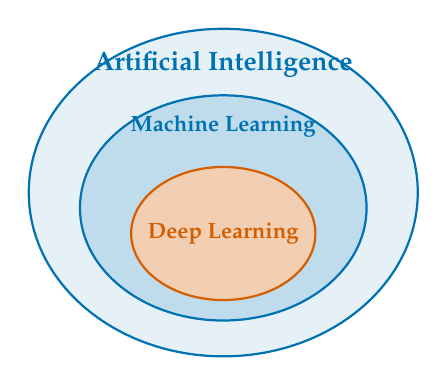
\begin{tikzpicture}[scale=0.65, every node/.style={scale=0.8}]
    \draw[fill=blue!10, draw=blue, thick] (0,0) ellipse (3.8cm and 3.2cm);
    \node[blue, font=\large\bfseries] at (0, 2.5) {Artificial Intelligence};

    \draw[fill=blue!25, draw=blue, thick] (0,-0.3) ellipse (2.8cm and 2.2cm);
    \node[blue, font=\bfseries] at (0, 1.3) {Machine Learning};

    \draw[fill=red!30, draw=red, thick] (0,-0.8) ellipse (1.8cm and 1.3cm);
    \node[red, font=\bfseries] at (0, -0.8) {Deep Learning};
\end{tikzpicture}
\end{center}
\end{column}
\end{columns}
\end{frame}

% ---- Why Now ----
\begin{frame}
\frametitle{Why Deep Learning Now?}

Three ingredients came together:

\vspace{6pt}
\begin{columns}[T]
\begin{column}{0.32\textwidth}
\centering
\textcolor{blue}{\textbf{1. Data}}\\[6pt]
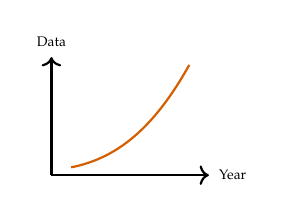
\begin{tikzpicture}[scale=0.5]
    \draw[thick, ->] (0,0) -- (4,0) node[right] {\tiny Year};
    \draw[thick, ->] (0,0) -- (0,3) node[above] {\tiny Data};
    \draw[thick, red] (0.5, 0.2) .. controls (1.5, 0.4) and (2.5, 1.0) .. (3.5, 2.8);
\end{tikzpicture}
\\[4pt]
{\small Internet, digitization, sensors, satellites}
\end{column}

\begin{column}{0.32\textwidth}
\centering
\textcolor{blue}{\textbf{2. Compute (GPUs)}}\\[6pt]
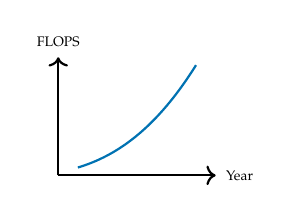
\begin{tikzpicture}[scale=0.5]
    \draw[thick, ->] (0,0) -- (4,0) node[right] {\tiny Year};
    \draw[thick, ->] (0,0) -- (0,3) node[above] {\tiny FLOPS};
    \draw[thick, blue] (0.5, 0.2) .. controls (1.5, 0.5) and (2.5, 1.2) .. (3.5, 2.8);
\end{tikzpicture}
\\[4pt]
{\small NVIDIA GPUs, Google TPUs, cloud computing}
\end{column}

\begin{column}{0.32\textwidth}
\centering
\textcolor{blue}{\textbf{3. Algorithms}}\\[6pt]
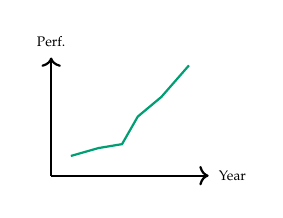
\begin{tikzpicture}[scale=0.5]
    \draw[thick, ->] (0,0) -- (4,0) node[right] {\tiny Year};
    \draw[thick, ->] (0,0) -- (0,3) node[above] {\tiny Perf.};
    \draw[thick, green] (0.5, 0.5) -- (1.2, 0.7) -- (1.8, 0.8) -- (2.2, 1.5) -- (2.8, 2.0) -- (3.5, 2.8);
\end{tikzpicture}
\\[4pt]
{\small Backpropagation, ReLU, dropout, Transformers}
\end{column}
\end{columns}

\vspace{10pt}
\begin{center}
\textcolor{red}{Neural networks existed since the 1950s --- what changed is the scale.}
\end{center}
\end{frame}

% ---- Brief History ----
\begin{frame}
\frametitle{A Brief History of Neural Networks}
\begin{center}
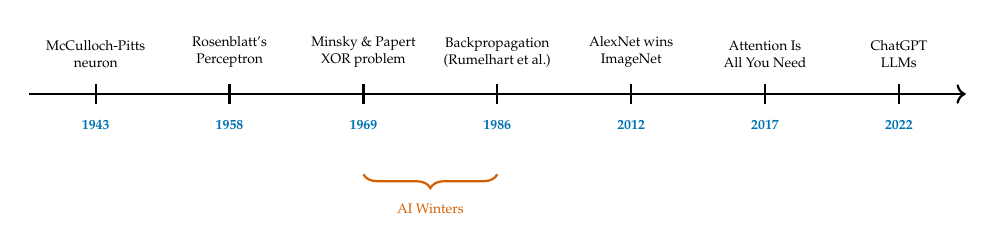
\begin{tikzpicture}[scale=0.85]
    \draw[thick, ->] (0,0) -- (14,0);

    % 1943
    \draw[thick] (1, -0.15) -- (1, 0.15);
    \node[below, font=\tiny\bfseries, text=blue] at (1, -0.25) {1943};
    \node[above, align=center, font=\tiny] at (1, 0.25) {McCulloch-Pitts\\neuron};
    % 1958
    \draw[thick] (3, -0.15) -- (3, 0.15);
    \node[below, font=\tiny\bfseries, text=blue] at (3, -0.25) {1958};
    \node[above, align=center, font=\tiny] at (3, 0.25) {Rosenblatt's\\Perceptron};
    % 1969
    \draw[thick] (5, -0.15) -- (5, 0.15);
    \node[below, font=\tiny\bfseries, text=blue] at (5, -0.25) {1969};
    \node[above, align=center, font=\tiny] at (5, 0.25) {Minsky \& Papert\\XOR problem};
    % 1986
    \draw[thick] (7, -0.15) -- (7, 0.15);
    \node[below, font=\tiny\bfseries, text=blue] at (7, -0.25) {1986};
    \node[above, align=center, font=\tiny] at (7, 0.25) {Backpropagation\\(Rumelhart et al.)};
    % 2012
    \draw[thick] (9, -0.15) -- (9, 0.15);
    \node[below, font=\tiny\bfseries, text=blue] at (9, -0.25) {2012};
    \node[above, align=center, font=\tiny] at (9, 0.25) {AlexNet wins\\ImageNet};
    % 2017
    \draw[thick] (11, -0.15) -- (11, 0.15);
    \node[below, font=\tiny\bfseries, text=blue] at (11, -0.25) {2017};
    \node[above, align=center, font=\tiny] at (11, 0.25) {Attention Is\\All You Need};
    % 2022
    \draw[thick] (13, -0.15) -- (13, 0.15);
    \node[below, font=\tiny\bfseries, text=blue] at (13, -0.25) {2022};
    \node[above, align=center, font=\tiny] at (13, 0.25) {ChatGPT\\LLMs};

    \draw[decorate, decoration={brace, amplitude=5pt, mirror}, thick, red] (5, -1.2) -- (7, -1.2);
    \node[below, text=red, font=\tiny] at (6, -1.5) {AI Winters};
\end{tikzpicture}
\end{center}

\vspace{4pt}
\begin{wideitemize}
    \item \textbf{1943--1969:} Early excitement $\to$ crushed by XOR limitation.
    \item \textbf{1986:} Backpropagation revives interest, but limited by compute.
    \item \textbf{2012:} Deep CNNs dominate computer vision (AlexNet).
    \item \textbf{2017--now:} Transformers $\to$ LLMs $\to$ foundation models revolution.
\end{wideitemize}
\end{frame}

% ---- DL in Economics ----

% ---- Course Roadmap ----
% ============================================================


% ---- Supervised Learning Setup ----

% ---- Regression vs Classification ----

% ---- Connection to Econometrics ----

% ---- Hypothesis Set ----

% ---- Training vs Test ----

% ---- Overfitting ----
% ============================================================


% ---- Linear Regression ----

% ---- Logistic Regression ----

% ---- Cross-Entropy ----

% ---- Gradient Descent ----

% ---- Gradient Derivation ----

% ---- Learning Rate ----

% ---- Limitation ----
\begin{frame}
\frametitle{The Limitation of Linear Models}

Linear models can only produce \textbf{linear decision boundaries}.

\begin{center}
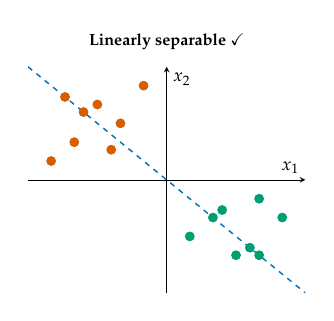
\begin{tikzpicture}[scale=0.65]
    \begin{axis}[
        xlabel={$x_1$}, ylabel={$x_2$},
        xmin=-3, xmax=3, ymin=-3, ymax=3,
        width=7cm, height=6cm,
        axis lines=middle, ticks=none,
        title={\small\textbf{Linearly separable} $\checkmark$}
    ]
    \addplot[only marks, mark=*, mark size=2.5pt, red] coordinates {
        (-2,1) (-1.5,2) (-2.5,0.5) (-1,1.5) (-0.5,2.5) (-1.8,1.8) (-2.2,2.2) (-1.2,0.8)
    };
    \addplot[only marks, mark=*, mark size=2.5pt, green] coordinates {
        (1,-1) (1.5,-2) (2,-0.5) (0.5,-1.5) (2.5,-1) (1.8,-1.8) (1.2,-0.8) (2,-2)
    };
    \addplot[thick, blue, dashed, domain=-3:3] {-x};
    \end{axis}
\end{tikzpicture}
\hspace{1cm}
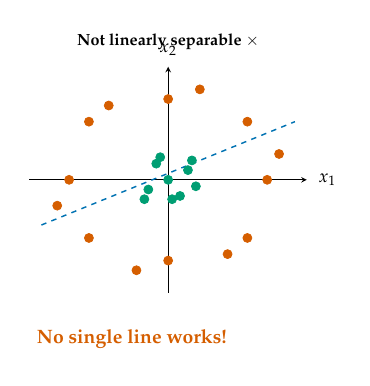
\begin{tikzpicture}[scale=0.65]
    \begin{axis}[
        xlabel={$x_1$}, ylabel={$x_2$},
        xmin=-3.5, xmax=3.5, ymin=-3.5, ymax=3.5,
        width=7cm, height=6cm,
        axis lines=middle, ticks=none,
        title={\small\textbf{Not linearly separable} $\times$},
        xlabel style={anchor=west, at={(axis description cs:1.02,0.5)}},
        ylabel style={anchor=south, at={(axis description cs:0.5,1.02)}}
    ]
    \addplot[only marks, mark=*, mark size=2.5pt, red] coordinates {
        (2.5,0) (-2.5,0) (0,2.5) (0,-2.5) (2,1.8) (-2,1.8) (2,-1.8) (-2,-1.8)
        (2.8,0.8) (-2.8,-0.8) (0.8,2.8) (-0.8,-2.8) (1.5,-2.3) (-1.5,2.3)
    };
    \addplot[only marks, mark=*, mark size=2.5pt, green] coordinates {
        (0,0) (0.5,0.3) (-0.3,0.5) (0.3,-0.5) (-0.5,-0.3) (0.7,-0.2) (-0.2,0.7) (0.1,-0.6) (-0.6,-0.6) (0.6,0.6)
    };
    \addplot[thick, blue, dashed, domain=-3.2:3.2] {0.5*x + 0.2};
    \end{axis}
    \node[font=\scriptsize\bfseries, text=red] at (2.0, -0.9) {No single line works!};
\end{tikzpicture}
\end{center}

\vspace{4pt}
\begin{center}
\textcolor{red}{We need \textbf{non-linear} models. This is where neural networks come in.}
\end{center}
\end{frame}


% ============================================================
\section{The Perceptron}
% ============================================================

\begin{transitionframe}
\begin{center}
{\Huge \textbf{The Perceptron}}
\end{center}
\end{transitionframe}

% ---- Biological Neuron ----
\begin{frame}
\frametitle{Biological Inspiration}

\begin{columns}[T]
\begin{column}{0.45\textwidth}
\textbf{Biological neuron:}
\begin{wideitemize}
    \item Receives input signals from \textbf{dendrites}.
    \item Processes them in the \textbf{cell body}.
    \item If total signal exceeds a threshold, \textbf{fires} through the \textbf{axon}.
    \item Connections have different \textbf{strengths} (synaptic weights).
\end{wideitemize}

\vspace{6pt}
{\small McCulloch \& Pitts (1943) proposed the first mathematical model of a neuron.}
\end{column}

\begin{column}{0.52\textwidth}
\begin{center}
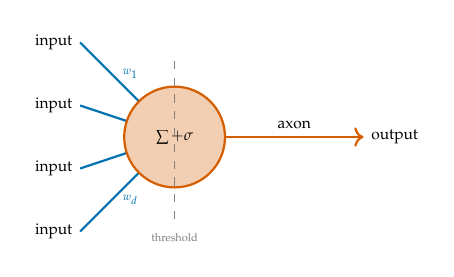
\begin{tikzpicture}[scale=0.8, every node/.style={scale=0.8}]
    \foreach \y in {-1.5, -0.5, 0.5, 1.5} {
        \draw[thick, blue] (-3, \y) -- (-1.5, 0);
        \node[left, font=\scriptsize] at (-3, \y) {input};
    }

    \draw[fill=red!30, draw=red, thick] (-1.5,0) circle (0.8cm);
    \node[font=\scriptsize\bfseries] at (-1.5, 0) {$\sum + \sigma$};

    \draw[thick, red, ->] (-0.7, 0) -- (1.5, 0);
    \node[above, font=\scriptsize] at (0.4, 0) {axon};

    \node[right, font=\scriptsize] at (1.5, 0) {output};

    \node[above, font=\tiny, blue] at (-2.2, 0.8) {$w_1$};
    \node[below, font=\tiny, blue] at (-2.2, -0.8) {$w_d$};

    \draw[dashed, gray] (-1.5, -1.3) -- (-1.5, 1.3);
    \node[below, font=\tiny, gray] at (-1.5, -1.4) {threshold};
\end{tikzpicture}
\end{center}

\vspace{6pt}
\begin{center}
\small The analogy is \textbf{loose}. Real neurons are far more complex. But the abstraction is powerful.
\end{center}
\end{column}
\end{columns}
\end{frame}

% ---- Artificial Neuron ----
\begin{frame}
\frametitle{The Artificial Neuron (Perceptron)}

\begin{center}
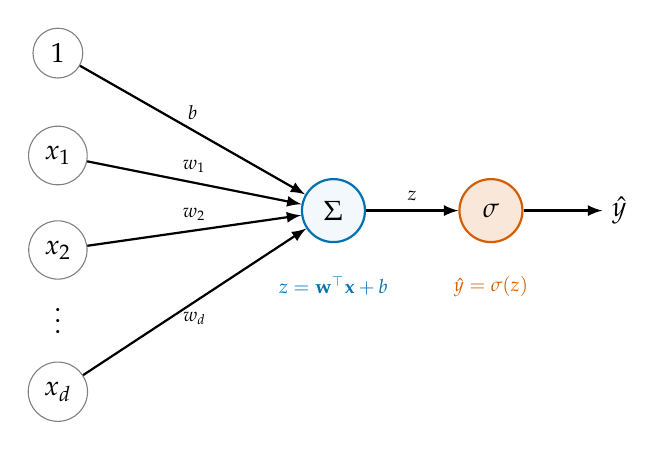
\begin{tikzpicture}[
    node distance=1.2cm and 1.8cm,
    neuron/.style={circle, draw=blue, thick, minimum size=0.8cm, fill=blue!5},
    input/.style={circle, draw=gray, minimum size=0.6cm},
    >=latex
]
    \node[input] (b) at (0, 2.5) {$1$};
    \node[input] (x1) at (0, 1.2) {$x_1$};
    \node[input] (x2) at (0, 0) {$x_2$};
    \node at (0, -0.8) {$\vdots$};
    \node[input] (xd) at (0, -1.8) {$x_d$};

    \node[neuron] (sum) at (3.5, 0.5) {$\Sigma$};

    \node[neuron, fill=red!15, draw=red] (act) at (5.5, 0.5) {$\sigma$};

    \node[right=1cm of act, font=\bfseries] (out) {$\hat{y}$};

    \draw[->, thick] (b) -- node[above, font=\scriptsize] {$b$} (sum);
    \draw[->, thick] (x1) -- node[above, font=\scriptsize] {$w_1$} (sum);
    \draw[->, thick] (x2) -- node[above, font=\scriptsize] {$w_2$} (sum);
    \draw[->, thick] (xd) -- node[below, font=\scriptsize] {$w_d$} (sum);

    \draw[->, thick] (sum) -- node[above, font=\scriptsize] {$z$} (act);

    \draw[->, thick] (act) -- (out);

    \node[below=0.3cm of sum, font=\scriptsize, blue] {$z = \vw^\top\vx + b$};
    \node[below=0.3cm of act, font=\scriptsize, red] {$\hat{y} = \sigma(z)$};
\end{tikzpicture}
\end{center}

\begin{tikzpicture}
\node [mybox] (box){%
    \begin{minipage}{0.93\textwidth}
    \[
        \hat{y} = \sigma\!\left(\sum_{j=1}^{d} w_j x_j + b\right) = \sigma(\vw^\top \vx + b)
    \]
    \begin{itemize}
        \item $\vx \in \R^d$: input features. \quad $\vw \in \R^d$: learnable weights. \quad $b \in \R$: bias.
        \item $\sigma(\cdot)$: \textbf{activation function} (introduces non-linearity).
    \end{itemize}
    \end{minipage}
};
\node[fancytitle, right=10pt] at (box.north west) {The Perceptron};
\end{tikzpicture}
\end{frame}

% ---- Activation Functions ----
\begin{frame}
\frametitle{Activation Functions}

The activation function $\sigma$ introduces \textbf{non-linearity} into the model.

\vspace{4pt}
\begin{center}
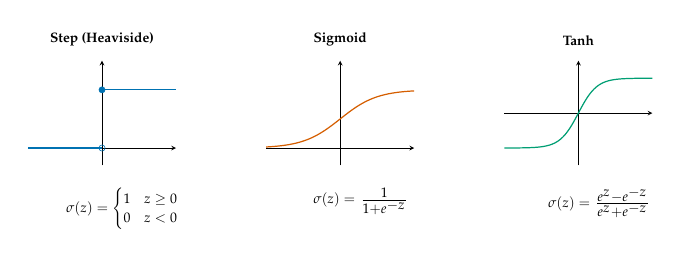
\begin{tikzpicture}[scale=0.55]
    \begin{scope}[shift={(0,0)}]
        \begin{axis}[
            title={\small\textbf{Step (Heaviside)}},
            width=5cm, height=4cm,
            xmin=-4, xmax=4, ymin=-0.3, ymax=1.5,
            axis lines=middle, ticks=none
        ]
        \addplot[thick, blue, domain=-4:0] {0};
        \addplot[thick, blue, domain=0:4] {1};
        \addplot[only marks, mark=*, mark size=2pt, blue] coordinates {(0,1)};
        \addplot[only marks, mark=o, mark size=2pt, blue] coordinates {(0,0)};
        \end{axis}
        \node[below, font=\tiny] at (2.2, -0.3) {$\sigma(z) = \begin{cases}1 & z \geq 0 \\ 0 & z < 0\end{cases}$};
    \end{scope}

    \begin{scope}[shift={(5.5,0)}]
        \begin{axis}[
            title={\small\textbf{Sigmoid}},
            width=5cm, height=4cm,
            xmin=-4, xmax=4, ymin=-0.3, ymax=1.5,
            axis lines=middle, ticks=none
        ]
        \addplot[thick, red, domain=-4:4, samples=100] {1/(1+exp(-x))};
        \end{axis}
        \node[below, font=\tiny] at (2.2, -0.3) {$\sigma(z) = \frac{1}{1+e^{-z}}$};
    \end{scope}

    \begin{scope}[shift={(11,0)}]
        \begin{axis}[
            title={\small\textbf{Tanh}},
            width=5cm, height=4cm,
            xmin=-4, xmax=4, ymin=-1.5, ymax=1.5,
            axis lines=middle, ticks=none
        ]
        \addplot[thick, green, domain=-4:4, samples=100] {tanh(x)};
        \end{axis}
        \node[below, font=\tiny] at (2.2, -0.3) {$\sigma(z) = \frac{e^z - e^{-z}}{e^z + e^{-z}}$};
    \end{scope}
\end{tikzpicture}

\vspace{8pt}
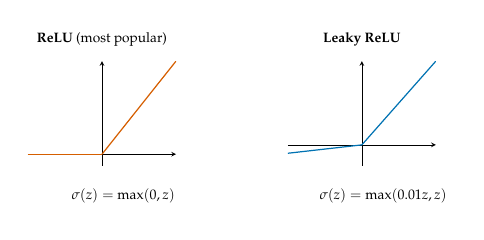
\begin{tikzpicture}[scale=0.55]
    \begin{scope}[shift={(2.5,0)}]
        \begin{axis}[
            title={\small\textbf{ReLU} (most popular)},
            width=5cm, height=4cm,
            xmin=-4, xmax=4, ymin=-0.5, ymax=4,
            axis lines=middle, ticks=none
        ]
        \addplot[thick, red, domain=-4:0] {0};
        \addplot[thick, red, domain=0:4] {x};
        \end{axis}
        \node[below, font=\tiny] at (2.2, -0.3) {$\sigma(z) = \max(0, z)$};
    \end{scope}

    \begin{scope}[shift={(8.5,0)}]
        \begin{axis}[
            title={\small\textbf{Leaky ReLU}},
            width=5cm, height=4cm,
            xmin=-4, xmax=4, ymin=-1, ymax=4,
            axis lines=middle, ticks=none
        ]
        \addplot[thick, blue, domain=-4:0] {0.1*x};
        \addplot[thick, blue, domain=0:4] {x};
        \end{axis}
        \node[below, font=\tiny] at (2.2, -0.3) {$\sigma(z) = \max(0.01z, z)$};
    \end{scope}
\end{tikzpicture}
\end{center}
\end{frame}

% ---- Why Non-linearity ----
\begin{frame}
\frametitle{Why Do We Need Non-linearity?}

\textcolor{red}{\textbf{Critical Insight:}} Without activation functions, a multi-layer network collapses to a \textbf{single linear transformation}.

\vspace{6pt}
\textbf{Proof:} Consider two linear layers (no activation):
\begin{align*}
    \vh^{(1)} &= \vW^{(1)}\vx + \vb^{(1)} \\
    \hat{\vy} &= \vW^{(2)}\vh^{(1)} + \vb^{(2)} = \vW^{(2)}(\vW^{(1)}\vx + \vb^{(1)}) + \vb^{(2)}
\end{align*}

\[
    = \underbrace{\vW^{(2)}\vW^{(1)}}_{\vW'}\vx + \underbrace{\vW^{(2)}\vb^{(1)} + \vb^{(2)}}_{\vb'} = \vW'\vx + \vb'
\]

\vspace{4pt}
This is just \textbf{another linear model}! The depth is useless.

\vspace{8pt}
\begin{center}
\fbox{\textbf{Non-linear activations are what make depth meaningful.}}
\end{center}

\vspace{6pt}
With activations: $\hat{\vy} = \vW^{(2)}\sigma(\vW^{(1)}\vx + \vb^{(1)}) + \vb^{(2)}$ \quad $\Rightarrow$ \textcolor{red}{genuinely non-linear}.
\end{frame}

% ---- XOR Problem ----
\begin{frame}
\frametitle{The XOR Problem: Why One Layer Is Not Enough}

\textbf{Boolean operations with a single perceptron:}

\begin{center}
\begin{tikzpicture}[scale=0.6]
    \begin{scope}[shift={(0,0)}]
        \begin{axis}[
            title={\small\textbf{AND} $\checkmark$},
            width=5cm, height=5cm,
            xmin=-0.6, xmax=1.6, ymin=-0.6, ymax=1.6,
            axis lines=middle, ticks=none,
            xtick={0,1}, ytick={0,1},
            xlabel={\tiny $x_1$}, ylabel={\tiny $x_2$},
            xlabel style={anchor=west, at={(axis description cs:1.02,0.25)}},
            ylabel style={anchor=south, at={(axis description cs:0.25,1.02)}}
        ]
        \addplot[only marks, mark=*, mark size=4pt, red] coordinates {(0,0) (0,1) (1,0)};
        \addplot[only marks, mark=*, mark size=4pt, green] coordinates {(1,1)};
        \addplot[thick, blue, dashed, domain=0.2:1.3] {-x + 1.5};
        \end{axis}
    \end{scope}

    \begin{scope}[shift={(6,0)}]
        \begin{axis}[
            title={\small\textbf{OR} $\checkmark$},
            width=5cm, height=5cm,
            xmin=-0.6, xmax=1.6, ymin=-0.6, ymax=1.6,
            axis lines=middle, ticks=none,
            xtick={0,1}, ytick={0,1},
            xlabel={\tiny $x_1$}, ylabel={\tiny $x_2$},
            xlabel style={anchor=west, at={(axis description cs:1.02,0.25)}},
            ylabel style={anchor=south, at={(axis description cs:0.25,1.02)}}
        ]
        \addplot[only marks, mark=*, mark size=4pt, red] coordinates {(0,0)};
        \addplot[only marks, mark=*, mark size=4pt, green] coordinates {(0,1) (1,0) (1,1)};
        \addplot[thick, blue, dashed, domain=-0.3:0.8] {-x + 0.5};
        \end{axis}
    \end{scope}

    \begin{scope}[shift={(12,0)}]
        \begin{axis}[
            title={\small\textbf{XOR} $\times$},
            width=5cm, height=5cm,
            xmin=-0.6, xmax=1.6, ymin=-0.6, ymax=1.6,
            axis lines=middle, ticks=none,
            xtick={0,1}, ytick={0,1},
            xlabel={\tiny $x_1$}, ylabel={\tiny $x_2$},
            xlabel style={anchor=west, at={(axis description cs:1.02,0.25)}},
            ylabel style={anchor=south, at={(axis description cs:0.25,1.02)}}
        ]
        \addplot[only marks, mark=*, mark size=4pt, red] coordinates {(0,0) (1,1)};
        \addplot[only marks, mark=*, mark size=4pt, green] coordinates {(0,1) (1,0)};
        \end{axis}
        \node[font=\scriptsize\bfseries, text=red] at (1.25, -2.5) {No single line!};
    \end{scope}
\end{tikzpicture}
\end{center}

\vspace{4pt}
\begin{wideitemize}
    \item AND and OR are \textbf{linearly separable} --- a single perceptron can learn them.
    \item XOR is \textbf{not linearly separable} --- requires composing multiple linear boundaries.
    \item Shown by \textbf{Minsky \& Papert (1969)} and caused the first ``AI winter''.
\end{wideitemize}
\end{frame}

% ---- Solving XOR (Part 1) ----
\begin{frame}
\frametitle{Solving XOR with Two Layers}

\textbf{Key insight:} XOR $= $ AND(OR($x_1, x_2$), NAND($x_1, x_2$))

\vspace{8pt}
\begin{center}
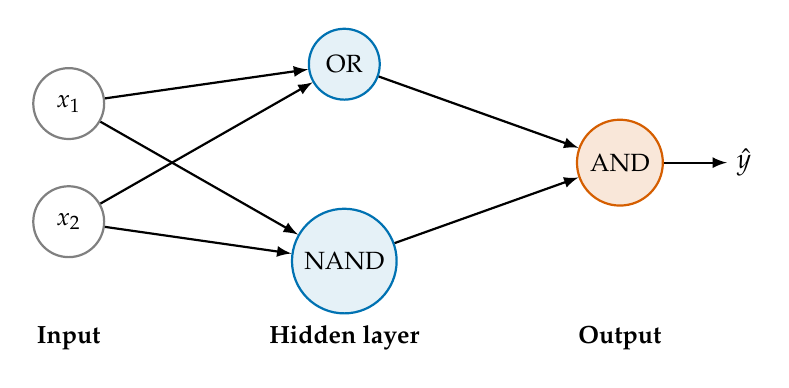
\begin{tikzpicture}[
    neuron/.style={circle, draw, thick, minimum size=0.9cm, font=\small},
    >=latex,
    scale=1
]
    \node[neuron, draw=gray] (x1) at (0, 1.5) {$x_1$};
    \node[neuron, draw=gray] (x2) at (0, 0) {$x_2$};

    \node[neuron, draw=blue, fill=blue!10] (h1) at (3.5, 2) {OR};
    \node[neuron, draw=blue, fill=blue!10] (h2) at (3.5, -0.5) {NAND};

    \node[neuron, draw=red, fill=red!15] (out) at (7, 0.75) {AND};

    \node[right=0.8cm of out, font=\bfseries] (y) {$\hat{y}$};

    \draw[->, thick] (x1) -- (h1);
    \draw[->, thick] (x1) -- (h2);
    \draw[->, thick] (x2) -- (h1);
    \draw[->, thick] (x2) -- (h2);
    \draw[->, thick] (h1) -- (out);
    \draw[->, thick] (h2) -- (out);
    \draw[->, thick] (out) -- (y);

    \node[below, font=\small\bfseries] at (0, -1.2) {Input};
    \node[below, font=\small\bfseries] at (3.5, -1.2) {Hidden layer};
    \node[below, font=\small\bfseries] at (7, -1.2) {Output};
\end{tikzpicture}
\end{center}

\vspace{8pt}
\begin{center}
\textcolor{red}{Adding one hidden layer solves the problem! This is the power of depth.}
\end{center}
\end{frame}

% ---- Solving XOR (Part 2 - truth table) ----
\begin{frame}
\frametitle{XOR: Truth Table Verification}

The hidden layer computes OR and NAND; the output layer applies AND.

\vspace{10pt}
\begin{center}
\renewcommand{\arraystretch}{1.4}
\begin{tabular}{cc|c|c|c}
    \toprule
    $x_1$ & $x_2$ & OR$(x_1,x_2)$ & NAND$(x_1,x_2)$ & AND(OR, NAND) = \textbf{XOR} \\
    \midrule
    0 & 0 & 0 & 1 & \textbf{0} \\
    0 & 1 & 1 & 1 & \textbf{1} \\
    1 & 0 & 1 & 1 & \textbf{1} \\
    1 & 1 & 1 & 0 & \textbf{0} \\
    \bottomrule
\end{tabular}
\end{center}

\vspace{10pt}
\begin{wideitemize}
    \item The hidden layer \textbf{transforms} the input into a new representation.
    \item In the new representation, the two classes \textbf{are} linearly separable.
    \item This is the essence of deep learning: \textcolor{red}{learn useful representations, then classify}.
\end{wideitemize}
\end{frame}

% ---- XOR Math ----
\begin{frame}
\frametitle{XOR: The Explicit Computation}

Using step activation $\sigma(z) = \mathbf{1}[z > 0]$:

\vspace{4pt}
\textbf{Hidden layer:}
\begin{align*}
    h_1 &= \sigma(x_1 + x_2 - 0.5) && \text{(OR: fires if $x_1 + x_2 > 0.5$)} \\
    h_2 &= \sigma(-x_1 - x_2 + 1.5) && \text{(NAND: fires if $x_1 + x_2 < 1.5$)}
\end{align*}

\textbf{Output layer:}
\[
    \hat{y} = \sigma(h_1 + h_2 - 1.5) \qquad \text{(AND: fires if $h_1 + h_2 > 1.5$)}
\]

\vspace{4pt}
\textbf{In matrix form:}
\[
    \vW^{(1)} = \begin{pmatrix} 1 & 1 \\ -1 & -1 \end{pmatrix}, \quad
    \vb^{(1)} = \begin{pmatrix} -0.5 \\ 1.5 \end{pmatrix}, \quad
    \vW^{(2)} = \begin{pmatrix} 1 & 1 \end{pmatrix}, \quad
    b^{(2)} = -1.5
\]

\vspace{4pt}
\textbf{Verify for $(x_1, x_2) = (1, 0)$:}
\[
    \vh = \sigma\!\left(\begin{pmatrix}1 & 1 \\ -1 & -1\end{pmatrix}\begin{pmatrix}1\\0\end{pmatrix} + \begin{pmatrix}-0.5\\1.5\end{pmatrix}\right) = \sigma\!\begin{pmatrix}0.5\\0.5\end{pmatrix} = \begin{pmatrix}1\\1\end{pmatrix}
\]
\[
    \hat{y} = \sigma(1 + 1 - 1.5) = \sigma(0.5) = 1 \quad \checkmark
\]
\end{frame}


% ============================================================
\section{From Perceptrons to Deep Networks}
% ============================================================

\begin{transitionframe}
\begin{center}
{\Huge \textbf{From Perceptrons to Deep Neural Networks}}
\end{center}
\end{transitionframe}

% ---- One Neuron to Layer ----
\begin{frame}
\frametitle{From One Neuron to a Layer}

\textbf{One neuron:} computes a single output feature
\[
    h_j = \sigma\!\left(\sum_{k=1}^{d} w_{jk}\, x_k + b_j\right) = \sigma(\vw_j^\top \vx + b_j)
\]

\textbf{A layer of $m$ neurons:} computes $m$ output features simultaneously
\[
    \vh = \sigma(\vW\vx + \vb) = \begin{pmatrix} \sigma(\vw_1^\top\vx + b_1) \\ \sigma(\vw_2^\top\vx + b_2) \\ \vdots \\ \sigma(\vw_m^\top\vx + b_m) \end{pmatrix} \in \R^m
\]

where $\vW \in \R^{m \times d}$ and $\vb \in \R^m$.

\vspace{6pt}
\begin{center}
\textcolor{red}{Each neuron in the layer learns a \textbf{different linear boundary}; the activation function makes each one non-linear.}
\end{center}
\end{frame}

% ---- Layer Diagram ----
\begin{frame}
\frametitle{A Fully Connected Layer}

\begin{center}
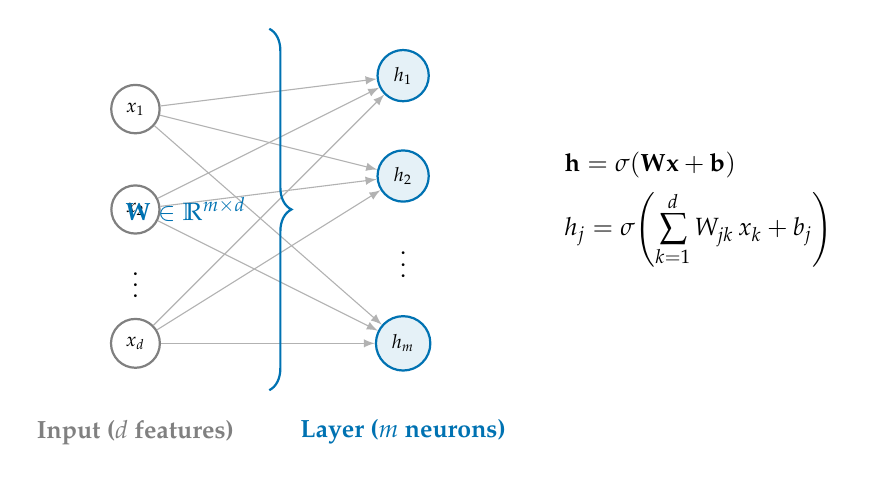
\begin{tikzpicture}[
    neuron/.style={circle, draw, thick, minimum size=0.6cm, font=\scriptsize},
    >=latex,
    scale=0.85
]
    \node[neuron, draw=gray] (i1) at (0, 3) {$x_1$};
    \node[neuron, draw=gray] (i2) at (0, 1.5) {$x_2$};
    \node at (0, 0.5) {\small$\vdots$};
    \node[neuron, draw=gray] (id) at (0, -0.5) {$x_d$};

    \node[neuron, fill=blue!10, draw=blue] (h1) at (4, 3.5) {$h_1$};
    \node[neuron, fill=blue!10, draw=blue] (h2) at (4, 2) {$h_2$};
    \node at (4, 0.8) {\small$\vdots$};
    \node[neuron, fill=blue!10, draw=blue] (hm) at (4, -0.5) {$h_m$};

    \foreach \i in {i1, i2, id} {
        \foreach \h in {h1, h2, hm} {
            \draw[->, thin, gray!60] (\i) -- (\h);
        }
    }

    \draw[decorate, decoration={brace, amplitude=8pt}, thick, blue]
        (2, 4.2) -- (2, -1.2);
    \node[blue, font=\small\bfseries, left] at (1.8, 1.5) {$\vW \in \R^{m \times d}$};

    \node[below, font=\small\bfseries, gray] at (0, -1.5) {Input ($d$ features)};
    \node[below, font=\small\bfseries, blue] at (4, -1.5) {Layer ($m$ neurons)};

    \node[right=1.5cm of hm, font=\small, align=left] at (4.5, 1.5) {
        $\vh = \sigma(\vW\vx + \vb)$\\[4pt]
        $h_j = \sigma\!\left(\displaystyle\sum_{k=1}^{d} W_{jk}\, x_k + b_j\right)$
    };
\end{tikzpicture}
\end{center}

\vspace{4pt}
\textbf{Every input is connected to every neuron:} this is called a \textbf{fully connected} (or \textbf{dense}) layer.

Parameters: $m \times d$ weights + $m$ biases $= m(d+1)$ total.
\end{frame}

% ---- Stacking Layers ----
\begin{frame}
\frametitle{Stacking Layers: The Deep Neural Network}

\textbf{A feedforward neural network} is a composition of layers:

\begin{tikzpicture}
\node [mybox] (box){%
    \begin{minipage}{0.93\textwidth}
    \begin{align*}
        \vh^{(0)} &= \vx && \text{(input)} \\
        \vh^{(1)} &= \sigma(\vW^{(1)}\vh^{(0)} + \vb^{(1)}) && \text{(hidden layer 1)} \\
        \vh^{(2)} &= \sigma(\vW^{(2)}\vh^{(1)} + \vb^{(2)}) && \text{(hidden layer 2)} \\
        &\;\;\vdots \\
        \vh^{(L-1)} &= \sigma(\vW^{(L-1)}\vh^{(L-2)} + \vb^{(L-1)}) && \text{(hidden layer $L-1$)} \\
        \hat{\vy} &= \vW^{(L)}\vh^{(L-1)} + \vb^{(L)} && \text{(output layer)}
    \end{align*}
    \end{minipage}
};
\node[fancytitle, right=10pt] at (box.north west) {Feedforward Neural Network with $L$ layers};
\end{tikzpicture}

\vspace{6pt}
\textbf{Terminology:}
\begin{wideitemize}
    \item \textbf{Depth:} number of layers $L$ (``deep'' $= L \geq 2$ hidden layers).
    \item \textbf{Width:} number of neurons per layer ($m^{(l)}$).
    \item \textbf{Parameters:} $\theta = \{\vW^{(1)}, \vb^{(1)}, \ldots, \vW^{(L)}, \vb^{(L)}\}$.
\end{wideitemize}
\end{frame}

% ---- Network Diagram ----
\begin{frame}
\frametitle{Deep Neural Network: Diagram}

\begin{center}
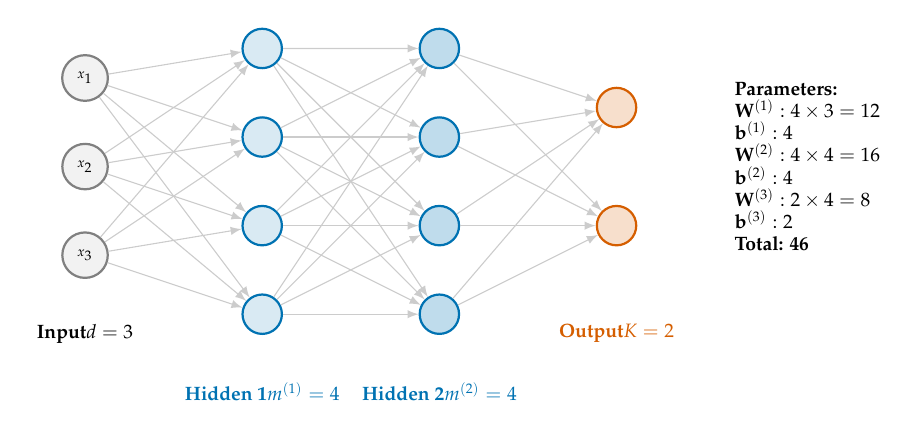
\begin{tikzpicture}[
    neuron/.style={circle, draw, thick, minimum size=0.5cm, font=\tiny},
    >=latex,
    scale=0.75
]
    \foreach \i/\y in {1/3, 2/1.5, 3/0} {
        \node[neuron, draw=gray, fill=gray!10] (i\i) at (0, \y) {$x_\i$};
    }
    \node[below, font=\scriptsize\bfseries] at (0, -1) {Input\\$d=3$};

    \foreach \i/\y in {1/3.5, 2/2, 3/0.5, 4/-1} {
        \node[neuron, fill=blue!15, draw=blue] (h1\i) at (3, \y) {};
    }
    \node[below, font=\scriptsize\bfseries, blue] at (3, -2) {Hidden 1\\$m^{(1)}=4$};

    \foreach \i/\y in {1/3.5, 2/2, 3/0.5, 4/-1} {
        \node[neuron, fill=blue!25, draw=blue] (h2\i) at (6, \y) {};
    }
    \node[below, font=\scriptsize\bfseries, blue] at (6, -2) {Hidden 2\\$m^{(2)}=4$};

    \foreach \i/\y in {1/2.5, 2/0.5} {
        \node[neuron, fill=red!20, draw=red] (o\i) at (9, \y) {};
    }
    \node[below, font=\scriptsize\bfseries, red] at (9, -1) {Output\\$K=2$};

    \foreach \i in {1,2,3} {
        \foreach \j in {1,2,3,4} {
            \draw[->, thin, gray!40] (i\i) -- (h1\j);
        }
    }

    \foreach \i in {1,2,3,4} {
        \foreach \j in {1,2,3,4} {
            \draw[->, thin, gray!40] (h1\i) -- (h2\j);
        }
    }

    \foreach \i in {1,2,3,4} {
        \foreach \j in {1,2} {
            \draw[->, thin, gray!40] (h2\i) -- (o\j);
        }
    }

    \node[right=1cm of o1, font=\scriptsize, align=left] at (9.5, 1.5) {
        \textbf{Parameters:}\\
        $\vW^{(1)}: 4 \times 3 = 12$\\
        $\vb^{(1)}: 4$\\
        $\vW^{(2)}: 4 \times 4 = 16$\\
        $\vb^{(2)}: 4$\\
        $\vW^{(3)}: 2 \times 4 = 8$\\
        $\vb^{(3)}: 2$\\
        \textbf{Total: 46}
    };
\end{tikzpicture}
\end{center}

\vspace{4pt}
\begin{center}
{\small Modern networks: GPT-4 has $\sim$1.8 \textbf{trillion} parameters. ResNet-50 has $\sim$25 million.}
\end{center}
\end{frame}

% ---- Forward Pass Example ----
\begin{frame}
\frametitle{Forward Pass: A Numerical Example}

\textbf{Network:} 2 inputs $\to$ 2 hidden (ReLU) $\to$ 1 output (linear)

\vspace{4pt}
\textbf{Given:} $\vx = \begin{pmatrix}1\\2\end{pmatrix}$, \;
$\vW^{(1)} = \begin{pmatrix}0.5 & -0.3\\0.2 & 0.8\end{pmatrix}$, \;
$\vb^{(1)} = \begin{pmatrix}0.1\\-0.1\end{pmatrix}$, \;
$\vW^{(2)} = \begin{pmatrix}0.6 & -0.4\end{pmatrix}$, \;
$b^{(2)} = 0.2$

\vspace{6pt}
\textbf{Step 1:} Compute hidden layer pre-activation
\[
    \vz^{(1)} = \vW^{(1)}\vx + \vb^{(1)} = \begin{pmatrix}0.5 & -0.3\\0.2 & 0.8\end{pmatrix}\begin{pmatrix}1\\2\end{pmatrix} + \begin{pmatrix}0.1\\-0.1\end{pmatrix} = \begin{pmatrix}-0.1\\1.7\end{pmatrix} + \begin{pmatrix}0.1\\-0.1\end{pmatrix} = \begin{pmatrix}0.0\\1.6\end{pmatrix}
\]

\textbf{Step 2:} Apply ReLU activation
\[
    \vh^{(1)} = \text{ReLU}(\vz^{(1)}) = \begin{pmatrix}\max(0, 0.0)\\\max(0, 1.6)\end{pmatrix} = \begin{pmatrix}0.0\\1.6\end{pmatrix}
\]

\textbf{Step 3:} Compute output
\[
    \hat{y} = \vW^{(2)}\vh^{(1)} + b^{(2)} = \begin{pmatrix}0.6 & -0.4\end{pmatrix}\begin{pmatrix}0.0\\1.6\end{pmatrix} + 0.2 = -0.64 + 0.2 = \textcolor{red}{-0.44}
\]
\end{frame}

% ---- Dimensions ----
\begin{frame}
\frametitle{Dimensions Cheat Sheet}

For a network with layers of widths $d = m^{(0)}, m^{(1)}, m^{(2)}, \ldots, m^{(L)}$:

\vspace{8pt}
\begin{center}
\renewcommand{\arraystretch}{1.5}
\begin{tabular}{llll}
    \toprule
    \textbf{Layer $l$} & \textbf{$\vW^{(l)}$} & \textbf{$\vb^{(l)}$} & \textbf{$\vh^{(l)}$} \\
    \midrule
    Input ($l=0$) & --- & --- & $\R^{m^{(0)}}$ \\
    Hidden $l$ & $\R^{m^{(l)} \times m^{(l-1)}}$ & $\R^{m^{(l)}}$ & $\R^{m^{(l)}}$ \\
    Output ($l=L$) & $\R^{m^{(L)} \times m^{(L-1)}}$ & $\R^{m^{(L)}}$ & $\R^{m^{(L)}}$ \\
    \bottomrule
\end{tabular}
\end{center}

\vspace{8pt}
\textbf{Total parameters:}
\[
    \sum_{l=1}^{L} \left( m^{(l)} \times m^{(l-1)} + m^{(l)} \right) = \sum_{l=1}^{L} m^{(l)}\left(m^{(l-1)} + 1\right)
\]

\vspace{4pt}
\textbf{Example:} Input $784$ $\to$ Hidden $256$ $\to$ Hidden $128$ $\to$ Output $10$
\[
    (256 \times 785) + (128 \times 257) + (10 \times 129) = 200{,}960 + 32{,}896 + 1{,}290 = \textcolor{red}{235{,}146}
\]
\end{frame}

% ---- What Does a Network Learn ----
\begin{frame}
\frametitle{What Does a Neural Network Learn?}

\textbf{Key idea:} each layer learns a \textcolor{red}{new representation} of the data.

\vspace{6pt}
\begin{center}
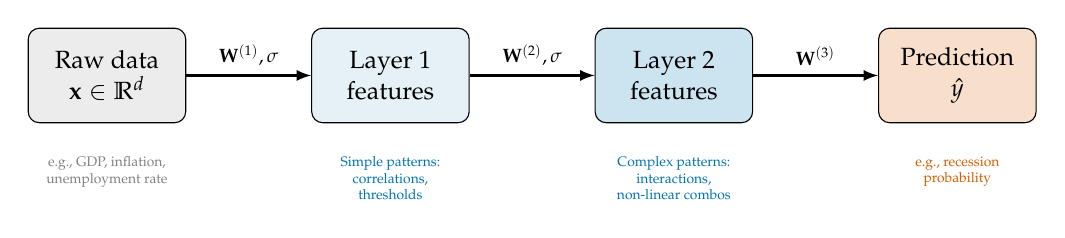
\begin{tikzpicture}[
    box/.style={rectangle, draw, rounded corners, minimum height=1.2cm, minimum width=2cm, align=center, font=\small},
    >=latex,
    scale=0.9
]
    \node[box, fill=gray!15] (raw) at (0,0) {Raw data\\$\vx \in \R^d$};
    \node[box, fill=blue!10] (h1) at (4,0) {Layer 1\\features};
    \node[box, fill=blue!20] (h2) at (8,0) {Layer 2\\features};
    \node[box, fill=red!20] (out) at (12,0) {Prediction\\$\hat{y}$};

    \draw[->, thick] (raw) -- node[above, font=\scriptsize] {$\vW^{(1)}, \sigma$} (h1);
    \draw[->, thick] (h1) -- node[above, font=\scriptsize] {$\vW^{(2)}, \sigma$} (h2);
    \draw[->, thick] (h2) -- node[above, font=\scriptsize] {$\vW^{(3)}$} (out);

    \node[below=0.3cm, font=\tiny, align=center, gray] at (raw.south) {e.g., GDP, inflation,\\unemployment rate};
    \node[below=0.3cm, font=\tiny, align=center, blue] at (h1.south) {Simple patterns:\\correlations,\\thresholds};
    \node[below=0.3cm, font=\tiny, align=center, blue] at (h2.south) {Complex patterns:\\interactions,\\non-linear combos};
    \node[below=0.3cm, font=\tiny, align=center, red] at (out.south) {e.g., recession\\probability};
\end{tikzpicture}
\end{center}

\vspace{6pt}
\textbf{For economists:} think of it as \textbf{automatic feature engineering}:
\begin{wideitemize}
    \item Instead of manually creating interaction terms ($x_1 \cdot x_2$, $x_1^2$, etc.).
    \item The network \textbf{learns} which transformations of the raw features are useful.
    \item Particularly powerful when $d$ is large (hundreds of variables).
\end{wideitemize}
\end{frame}


% ============================================================
\section{Introduction to PyTorch and Google Colab}
% ============================================================

\begin{transitionframe}
\begin{center}
{\Huge \textbf{Introduction to PyTorch \& Google Colab}}
\end{center}
\end{transitionframe}

% ---- PyTorch ----
\begin{frame}
\frametitle{Why PyTorch?}

\textbf{PyTorch} is the most widely used deep learning framework in research.

\vspace{6pt}
\begin{columns}[T]
\begin{column}{0.48\textwidth}
\textcolor{blue}{\textbf{Key features:}}
\begin{wideitemize}
    \item \textbf{Dynamic computation graphs} (define-by-run).
    \item \textbf{Automatic differentiation} (autograd).
    \item GPU acceleration (CUDA).
    \item Pythonic, intuitive API.
    \item Huge ecosystem (torchvision, torchtext, HuggingFace).
\end{wideitemize}
\end{column}

\begin{column}{0.48\textwidth}
\textcolor{blue}{\textbf{Alternatives:}}
\begin{itemize}
    \item TensorFlow / Keras (Google).
    \item JAX (Google Research).
    \item Flux.jl (Julia).
\end{itemize}

\vspace{6pt}
\textcolor{blue}{\textbf{We use PyTorch because:}}
\begin{itemize}
    \item Standard in academia.
    \item Best for learning DL concepts.
    \item HuggingFace integration (for LLMs).
\end{itemize}
\end{column}
\end{columns}
\end{frame}

% ---- Tensors ----
\begin{frame}[fragile]
\frametitle{PyTorch Tensors}

\textbf{Tensors} are the fundamental data structure --- like NumPy arrays but with GPU support.

\vspace{4pt}
\begin{lstlisting}
import torch

# Creating tensors
x = torch.tensor([1.0, 2.0, 3.0])          # 1D tensor (vector)
W = torch.randn(3, 2)                       # 2D tensor (matrix), random
b = torch.zeros(3)                          # 1D tensor of zeros

# Operations
z = W @ x + b                # Matrix-vector multiply + bias (@ = matmul)
print(z.shape)               # torch.Size([3])

# Move to GPU
device = torch.device('cuda' if torch.cuda.is_available() else 'cpu')
x_gpu = x.to(device)
W_gpu = W.to(device)
z_gpu = W_gpu @ x_gpu        # Computation happens on GPU!
\end{lstlisting}

\vspace{4pt}
\textbf{Key difference from NumPy:} tensors track computation for \textcolor{red}{automatic differentiation}.
\end{frame}

% ---- Autograd ----
\begin{frame}[fragile]
\frametitle{Automatic Differentiation (Autograd)}

PyTorch can automatically compute gradients --- the foundation of training neural networks.

\begin{lstlisting}
import torch

# Create tensors with gradient tracking
w = torch.tensor(2.0, requires_grad=True)
b = torch.tensor(1.0, requires_grad=True)
x = torch.tensor(3.0)
y_true = torch.tensor(7.0)     # target

# Forward pass: compute prediction and loss
y_pred = w * x + b             # y_pred = 2*3 + 1 = 7
loss = (y_true - y_pred) ** 2  # MSE for one sample = 0

# Backward pass: compute gradients
loss.backward()

# Gradients are now available!
print(w.grad)    # d(loss)/dw = 2*(y_true - y_pred)*(-x) = 0
print(b.grad)    # d(loss)/db = 2*(y_true - y_pred)*(-1) = 0
\end{lstlisting}

\vspace{4pt}
\textcolor{red}{\textbf{Key Insight:}} \texttt{loss.backward()} computes $\frac{\partial \mathcal{L}}{\partial w}$ and $\frac{\partial \mathcal{L}}{\partial b}$ \textbf{automatically} using the chain rule. We'll derive backpropagation in Lecture 2.
\end{frame}

% ---- Single Neuron ----
\begin{frame}[fragile]
\frametitle{Implementing a Single Neuron in PyTorch}

\begin{lstlisting}
import torch
import torch.nn as nn

# A single neuron: 2 inputs -> 1 output with sigmoid activation
class SingleNeuron(nn.Module):
    def __init__(self):
        super().__init__()
        self.linear = nn.Linear(2, 1)    # 2 inputs, 1 output
        self.sigmoid = nn.Sigmoid()

    def forward(self, x):
        z = self.linear(x)              # z = w^T x + b
        return self.sigmoid(z)          # sigma(z)

# Create the neuron and a sample input
neuron = SingleNeuron()
x = torch.tensor([[1.0, 2.0]])         # batch of 1, 2 features
y_pred = neuron(x)
print(f"Prediction: {y_pred.item():.4f}")

# Check parameters
for name, param in neuron.named_parameters():
    print(f"{name}: {param.data}")
\end{lstlisting}

\vspace{2pt}
{\small \texttt{nn.Linear(2, 1)} creates a layer with $\vW \in \R^{1\times 2}$ and $b \in \R$ (3 parameters total).}
\end{frame}

% ---- Training Loop ----
\begin{frame}[fragile]
\frametitle{The Training Loop (Preview)}

\begin{lstlisting}
# The basic training loop structure
model = SingleNeuron()
optimizer = torch.optim.SGD(model.parameters(), lr=0.01)  # SGD
criterion = nn.BCELoss()                                   # Binary CE

for epoch in range(100):
    # Forward pass
    y_pred = model(x_train)
    loss = criterion(y_pred, y_train)

    # Backward pass
    optimizer.zero_grad()    # Reset gradients to zero
    loss.backward()          # Compute gradients (backpropagation)

    # Update parameters
    optimizer.step()         # w <- w - alpha * grad

    if epoch % 10 == 0:
        print(f"Epoch {epoch}, Loss: {loss.item():.4f}")
\end{lstlisting}

\vspace{4pt}
\begin{center}
\textbf{Every DL training follows this pattern:} forward $\to$ loss $\to$ backward $\to$ update.

We'll understand \emph{exactly why} in Lecture 2 (backpropagation).
\end{center}
\end{frame}

% ---- Google Colab ----
\begin{frame}[fragile]
\frametitle{Google Colab Setup}

\begin{columns}[T]
\begin{column}{0.55\textwidth}
\textbf{Google Colab} provides free access to GPUs in the browser.

\vspace{6pt}
\textcolor{blue}{\textbf{Getting started:}}
\begin{enumerate}
    \item Go to \texttt{colab.research.google.com}.
    \item Create a new notebook.
    \item Runtime $\to$ Change runtime type $\to$ \textbf{GPU}.
    \item PyTorch is pre-installed!
\end{enumerate}

\vspace{6pt}
\textcolor{blue}{\textbf{Recommended subscriptions:}}
\begin{itemize}
    \item \textbf{Colab Pro} (\$10/mo): better GPUs, longer runtime.
    \item \textbf{Colab Pro+} (\$50/mo): even more resources.
    \item Free tier works for Lectures 1--5.
\end{itemize}
\end{column}

\begin{column}{0.42\textwidth}
\textbf{Verify GPU access:}

\vspace{4pt}
\begin{lstlisting}
import torch
print(torch.cuda.is_available())
# True
print(torch.cuda.get_device_name(0))
# Tesla T4
\end{lstlisting}

\vspace{6pt}
\textcolor{blue}{\textbf{Also recommended:}}
\begin{itemize}
    \item \textbf{Claude Code} (\$20/mo) for coding assistance.
    \item Use LLMs as a learning tool, not a replacement.
\end{itemize}
\end{column}
\end{columns}
\end{frame}


% ============================================================
\section{Summary and Next Steps}
% ============================================================

\begin{transitionframe}
\begin{center}
{\Huge \textbf{Summary \& Next Steps}}
\end{center}
\end{transitionframe}

% ---- Summary ----
\begin{frame}
\frametitle{Summary}

\begin{enumerate}
    \item \textbf{Supervised learning:} given data $\{(\vx_i, y_i)\}$, find $f$ that generalizes.

    \item \textbf{Linear models} (regression/logistic) are the starting point:
    \[
        f(\vx) = \vw^\top\vx + b \qquad \text{or} \qquad p(y=1|\vx) = \sigma(\vw^\top\vx + b)
    \]

    \item \textbf{Gradient descent} iteratively minimizes the loss:
    \[
        \vw \leftarrow \vw - \alpha \nabla_{\vw}\mathcal{L}
    \]

    \item \textbf{The perceptron} = linear model + activation function. Learns AND, OR but \textcolor{red}{not XOR}.

    \item \textbf{Deep neural networks} stack layers of perceptrons:
    \[
        \vh^{(l)} = \sigma(\vW^{(l)}\vh^{(l-1)} + \vb^{(l)})
    \]

    \item \textbf{Non-linear activations} (ReLU, sigmoid) are essential --- without them, depth is useless.

    \item \textbf{PyTorch} provides tensors + autograd for implementation.
\end{enumerate}
\end{frame}

% ---- Next Lecture ----

% ---- References ----




%%% TIKZ STUFF
\tikzset{
        every picture/.style={remember picture,baseline},
        every node/.style={anchor=base,align=center,outer sep=1.5pt},
        every path/.style={thick},
        }
\tikzstyle{every picture}+=[remember picture]
\tikzstyle{mybox} =[draw=black, very thick, rectangle, inner sep=10pt, inner ysep=20pt]
\tikzstyle{fancytitle} =[draw=black,fill=red, text=white]
%%%% END TIKZ STUFF

% ============================================================
% Title Slide
% ============================================================



% ============================================================
\section{Recap and Activation Functions Deep Dive}
% ============================================================

\begin{transitionframe}
\begin{center}
{\Huge \textbf{Recap \& Activation Functions}}
\end{center}
\end{transitionframe}

% ---- Recap ----

% ---- Activation Functions Revisited ----
\begin{frame}
\frametitle{Activation Functions: Derivatives Matter}

To do backpropagation, we need the \textbf{derivative} of each activation function.

\vspace{4pt}
\renewcommand{\arraystretch}{1.6}
\begin{center}
{\small
\begin{tabular}{llll}
\toprule
\textbf{Name} & \textbf{$\sigma(z)$} & \textbf{$\sigma'(z)$} & \textbf{Range} \\
\midrule
Sigmoid & $\frac{1}{1+e^{-z}}$ & $\sigma(z)(1 - \sigma(z))$ & $(0, 1)$ \\[3pt]
Tanh & $\frac{e^z - e^{-z}}{e^z + e^{-z}}$ & $1 - \tanh^2(z)$ & $(-1, 1)$ \\[3pt]
ReLU & $\max(0, z)$ & $1$ if $z > 0$; $0$ if $z < 0$ & $[0, \infty)$ \\[3pt]
Leaky ReLU & $\max(\alpha z, z)$ & $1$ if $z > 0$; $\alpha$ if $z < 0$ & $(-\infty, \infty)$ \\
\bottomrule
\end{tabular}
}
\end{center}
\end{frame}

% ---- Sigmoid Derivative ----
\begin{frame}
\frametitle{Deriving the Sigmoid Derivative}

Let $\sigma(z) = \frac{1}{1 + e^{-z}} = (1 + e^{-z})^{-1}$. Apply the chain rule:

\vspace{2pt}
\textbf{Step 1:}
$\sigma'(z) = -(1 + e^{-z})^{-2} \cdot (-e^{-z}) = \frac{e^{-z}}{(1 + e^{-z})^2}$

\vspace{4pt}
\textbf{Step 2:} Rewrite in terms of $\sigma(z)$:
\[
    \sigma'(z) = \frac{1}{1+e^{-z}} \cdot \frac{e^{-z}}{1+e^{-z}} = \sigma(z) \cdot \frac{(1 + e^{-z}) - 1}{1+e^{-z}} = \sigma(z)(1 - \sigma(z))
\]

\begin{tikzpicture}
\node [mybox] (box){%
    \begin{minipage}{0.93\textwidth}
    \vspace{-6pt}
    \[
        \boxed{\sigma'(z) = \sigma(z)\big(1 - \sigma(z)\big)}
    \]
    \vspace{-8pt}
    \textbf{Note:} Max value $\sigma'(0) = 0.25$. This causes the \textcolor{red}{vanishing gradient problem}.
    \end{minipage}
};
\node[fancytitle, right=10pt] at (box.north west) {Result};
\end{tikzpicture}
\end{frame}

% ---- Vanishing Gradient ----
\begin{frame}
\frametitle{The Vanishing Gradient Problem}

\begin{columns}[T]
\begin{column}{0.48\textwidth}
\textbf{Sigmoid derivative} peaks at $0.25$:

\begin{center}
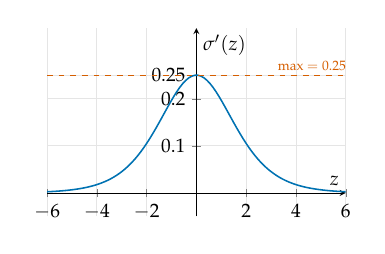
\begin{tikzpicture}[scale=0.7]
    \begin{axis}[
        xlabel={$z$}, ylabel={$\sigma'(z)$},
        xmin=-6, xmax=6, ymin=-0.05, ymax=0.35,
        width=7cm, height=5cm,
        axis lines=middle,
        grid=major, grid style={gray!20},
        ytick={0, 0.1, 0.2, 0.25},
    ]
    \addplot[thick, blue, domain=-6:6, samples=100] {exp(-x)/((1+exp(-x))^2)};
    \draw[dashed, red] (axis cs:-6,0.25) -- (axis cs:6,0.25);
    \node[right, font=\scriptsize, text=red] at (axis cs:3, 0.27) {max $= 0.25$};
    \end{axis}
\end{tikzpicture}
\end{center}
\end{column}

\begin{column}{0.48\textwidth}
\textbf{Problem for deep networks:}

With $L$ layers of sigmoid, the gradient at layer 1 involves:
\[
    \pd{\mathcal{L}}{\vW^{(1)}} \propto \prod_{l=1}^{L} \sigma'(z^{(l)})
\]

\vspace{4pt}
Since $\sigma'(z) \leq 0.25$:
\[
    \prod_{l=1}^{L} 0.25 = 0.25^L
\]

\vspace{4pt}
For $L = 10$: $0.25^{10} \approx 10^{-6}$

\vspace{6pt}
\textcolor{red}{\textbf{Gradients vanish exponentially with depth!}}
\end{column}
\end{columns}

\vspace{4pt}
\textbf{Solution:} Use \textbf{ReLU}, where $\sigma'(z) = 1$ for $z > 0$. No vanishing gradient!
\end{frame}

% ---- ReLU advantages ----
\begin{frame}
\frametitle{Why ReLU Dominates}

\begin{columns}[T]
\begin{column}{0.48\textwidth}
\begin{center}
\textcolor{blue}{\textbf{ReLU:}} $\sigma(z) = \max(0, z)$

\begin{tikzpicture}[scale=0.65]
    \begin{axis}[
        width=6cm, height=5cm,
        xmin=-4, xmax=4, ymin=-0.5, ymax=4,
        axis lines=middle, ticks=none,
        xlabel={$z$}, ylabel={$\sigma(z)$}
    ]
    \addplot[thick, red, domain=-4:0] {0};
    \addplot[thick, red, domain=0:4] {x};
    \end{axis}
\end{tikzpicture}
\end{center}

\begin{wideitemize}
    \item Derivative $= 1$ for $z > 0$: no vanishing gradient.
    \item Computationally cheap.
    \item Sparse activation (many neurons output 0).
\end{wideitemize}
\end{column}

\begin{column}{0.48\textwidth}
\begin{center}
\textcolor{blue}{\textbf{ReLU derivative:}}

\begin{tikzpicture}[scale=0.65]
    \begin{axis}[
        width=6cm, height=5cm,
        xmin=-4, xmax=4, ymin=-0.5, ymax=1.5,
        axis lines=middle, ticks=none,
        xlabel={$z$}, ylabel={$\sigma'(z)$}
    ]
    \addplot[thick, blue, domain=-4:-0.01] {0};
    \addplot[thick, blue, domain=0.01:4] {1};
    \addplot[only marks, mark=*, mark size=2pt, blue] coordinates {(0,0)};
    \end{axis}
\end{tikzpicture}
\end{center}

\textcolor{red}{\textbf{Problem:}} ``Dead ReLU'' --- if $z < 0$ always, the neuron never updates.

\vspace{6pt}
\textbf{Fix:} Leaky ReLU ($\alpha = 0.01$), ELU, GELU.
\end{column}
\end{columns}
\end{frame}

% ---- Softmax ----
\begin{frame}
\frametitle{Softmax: From Binary to Multi-class Classification}

For $K$ classes, we need a probability distribution over classes.

\begin{tikzpicture}
\node [mybox] (box){%
    \begin{minipage}{0.93\textwidth}
    Given logits $z_1, z_2, \ldots, z_K$ (raw outputs of the network), the \textbf{softmax} function computes:
    \[
        p(y = k | \vx) = \text{softmax}(z_k) = \frac{e^{z_k}}{\sum_{j=1}^{K} e^{z_j}} \qquad \text{for } k = 1, \ldots, K
    \]
    \end{minipage}
};
\node[fancytitle, right=10pt] at (box.north west) {Softmax Function};
\end{tikzpicture}

\vspace{6pt}
\textbf{Properties:}
\begin{wideitemize}
    \item $\sum_{k=1}^{K} p(y = k | \vx) = 1$ \quad (valid probability distribution).
    \item $p(y = k | \vx) > 0$ for all $k$ \quad (always positive).
    \item Larger $z_k$ $\Rightarrow$ higher probability for class $k$.
    \item When $K = 2$: softmax reduces to the sigmoid function.
\end{wideitemize}
\end{frame}

% ---- Softmax Example ----
\begin{frame}
\frametitle{Softmax: Numerical Example}

\textbf{Network output (logits)} for $K = 3$ classes:
\[
    \vz = \begin{pmatrix} z_1 \\ z_2 \\ z_3 \end{pmatrix} = \begin{pmatrix} 2.0 \\ 1.0 \\ 0.1 \end{pmatrix}
\]

\textbf{Step 1:} Compute exponentials:
\[
    e^{z_1} = e^{2.0} = 7.389, \quad e^{z_2} = e^{1.0} = 2.718, \quad e^{z_3} = e^{0.1} = 1.105
\]

\textbf{Step 2:} Sum of exponentials:
\[
    \sum_{j=1}^{3} e^{z_j} = 7.389 + 2.718 + 1.105 = 11.212
\]

\textbf{Step 3:} Normalize:
\[
    p_1 = \frac{7.389}{11.212} = \textcolor{red}{0.659}, \quad p_2 = \frac{2.718}{11.212} = 0.242, \quad p_3 = \frac{1.105}{11.212} = 0.099
\]

\vspace{4pt}
\textbf{Prediction:} class 1 with probability 65.9\%. \quad Check: $0.659 + 0.242 + 0.099 = 1.0$ \; $\checkmark$
\end{frame}


% ============================================================
\section{Loss Functions in Detail}
% ============================================================

\begin{transitionframe}
\begin{center}
{\Huge \textbf{Loss Functions in Detail}}
\end{center}
\end{transitionframe}

% ---- Loss Functions Overview ----
\begin{frame}
\frametitle{Loss Functions: Overview}

The loss function $\mathcal{L}$ measures how far our prediction $\hat{y}$ is from the truth $y$.

\vspace{8pt}
\renewcommand{\arraystretch}{1.6}
\begin{center}
\begin{tabular}{llll}
\toprule
\textbf{Task} & \textbf{Loss} & \textbf{Formula} & \textbf{Output activation} \\
\midrule
Regression & MSE & $\frac{1}{N}\sum(y_i - \hat{y}_i)^2$ & None (linear) \\
Binary classif.\ & BCE & $-\frac{1}{N}\sum[y\log\hat{y} + (1-y)\log(1-\hat{y})]$ & Sigmoid \\
Multi-class & CE & $-\frac{1}{N}\sum\sum y_{ik}\log \hat{y}_{ik}$ & Softmax \\
\bottomrule
\end{tabular}
\end{center}

\vspace{8pt}
\textbf{Key principle:} the choice of loss function depends on the task. The loss determines what the network optimizes for.
\end{frame}

% ---- MSE Gradient ----
\begin{frame}
\frametitle{MSE Loss: Gradient Derivation}

\textbf{Loss for one sample:} $\ell = (y - \hat{y})^2$ where $\hat{y} = f(\vx; \theta)$.

\vspace{6pt}
\textbf{Gradient with respect to the prediction:}
\[
    \pd{\ell}{\hat{y}} = \pd{}{\hat{y}}(y - \hat{y})^2 = 2(y - \hat{y}) \cdot (-1) = \textcolor{red}{-2(y - \hat{y})}
\]

\vspace{4pt}
\textbf{Average over $N$ samples:}
\[
    \pd{\mathcal{L}}{\hat{y}_i} = -\frac{2}{N}(y_i - \hat{y}_i)
\]

\vspace{6pt}
\textbf{Interpretation:}
\begin{wideitemize}
    \item The gradient is proportional to the \textbf{error} $(y_i - \hat{y}_i)$.
    \item Large errors produce large gradients $\Rightarrow$ faster learning.
    \item This is the \textbf{starting point} of backpropagation: we first compute $\pd{\mathcal{L}}{\hat{y}}$, then propagate backward.
\end{wideitemize}
\end{frame}

% ---- BCE Derivation ----
\begin{frame}
\frametitle{Binary Cross-Entropy: Derivation from MLE}

Assume $y \in \{0, 1\}$ and model predicts $\hat{y} = p(y=1|\vx)$. Likelihood of one sample:
$p(y | \vx) = \hat{y}^{y}(1 - \hat{y})^{1-y}$.

\vspace{2pt}
\textbf{Log-likelihood} $\to$ \textbf{Negative log-likelihood} (= BCE):
\[
    \ell = -\big[y \log \hat{y} + (1-y) \log(1 - \hat{y})\big]
\]

\textbf{Gradient w.r.t.\ $\hat{y}$:}
\[
    \pd{\ell}{\hat{y}} = -\frac{y}{\hat{y}} + \frac{1-y}{1-\hat{y}} = \frac{\hat{y} - y}{\hat{y}(1-\hat{y})}
\]

\textbf{Gradient w.r.t.\ logit $z$} (where $\hat{y} = \sigma(z)$, $\sigma' = \sigma(1-\sigma)$):
\[
    \pd{\ell}{z} = \pd{\ell}{\hat{y}} \cdot \sigma'(z) = \frac{\hat{y} - y}{\hat{y}(1-\hat{y})} \cdot \hat{y}(1-\hat{y}) = \textcolor{red}{\hat{y} - y}
\]
\end{frame}

% ---- BCE Gradient Beauty ----
\begin{frame}
\frametitle{The Beautiful Cancellation: BCE + Sigmoid}

\begin{tikzpicture}
\node [mybox] (box){%
    \begin{minipage}{0.93\textwidth}
    \vspace{-6pt}
    \[
        \pd{\ell}{z} = \sigma(z) - y = \hat{y} - y
    \]
    \vspace{-8pt}
    The gradient of BCE w.r.t.\ the logit $z$ is simply $\hat{y} - y$.
    \end{minipage}
};
\node[fancytitle, right=10pt] at (box.north west) {Key Result};
\end{tikzpicture}

\vspace{6pt}
\textbf{Why is this beautiful?}
\begin{itemize}
    \item No $\sigma'(z)$ term in the gradient!
    \item Even when sigmoid saturates, gradient is large if prediction is wrong.
    \item \textbf{Not a coincidence:} BCE was designed to pair with sigmoid.
    \item Compare: MSE + sigmoid $\Rightarrow \pd{\ell}{z} = -2(y - \hat{y})\sigma'(z)$ -- vanishes!
\end{itemize}

\textbf{Lesson:} \textcolor{red}{Always pair the right loss with the right activation.}
\end{frame}

% ---- Categorical Cross-Entropy ----
\begin{frame}
\frametitle{Categorical Cross-Entropy Loss}

For $K$-class classification with one-hot encoding $\vy = (y_1, \ldots, y_K)$:

\begin{tikzpicture}
\node [mybox] (box){%
    \begin{minipage}{0.93\textwidth}
    \[
        \mathcal{L} = -\sum_{k=1}^{K} y_k \log \hat{y}_k = -\log \hat{y}_c
    \]
    where $c$ is the true class (since only $y_c = 1$, all other $y_k = 0$).
    \end{minipage}
};
\node[fancytitle, right=10pt] at (box.north west) {Categorical Cross-Entropy};
\end{tikzpicture}

\vspace{6pt}
\textbf{Example:} True class $= 2$ (i.e., $\vy = (0, 1, 0)$), predictions $\hat{\vy} = (0.1, 0.7, 0.2)$:
\[
    \mathcal{L} = -(0 \cdot \log 0.1 + 1 \cdot \log 0.7 + 0 \cdot \log 0.2) = -\log(0.7) = 0.357
\]

\vspace{4pt}
If predictions were $\hat{\vy} = (0.1, 0.95, 0.05)$:
\[
    \mathcal{L} = -\log(0.95) = 0.051 \quad \text{(much lower --- better prediction)}
\]

\vspace{6pt}
\textbf{Interpretation:} The loss only depends on the \textbf{predicted probability for the correct class}.
\end{frame}

% ---- Softmax Jacobian ----
\begin{frame}
\frametitle{Softmax + Cross-Entropy: Gradient (Step 1)}

Let $\hat{y}_k = \text{softmax}(z_k) = \frac{e^{z_k}}{\sum_j e^{z_j}}$ and $\mathcal{L} = -\sum_k y_k \log \hat{y}_k$.

\vspace{6pt}
\textbf{We want:} $\pd{\mathcal{L}}{z_i}$ for each logit $z_i$. First, compute the \textbf{Jacobian of softmax}:

\vspace{4pt}
\textbf{Case $i = k$:}
\[
    \pd{\hat{y}_k}{z_k} = \frac{e^{z_k}\sum_j e^{z_j} - e^{z_k} \cdot e^{z_k}}{(\sum_j e^{z_j})^2} = \hat{y}_k - \hat{y}_k^2 = \hat{y}_k(1 - \hat{y}_k)
\]

\textbf{Case $i \neq k$:}
\[
    \pd{\hat{y}_k}{z_i} = \frac{0 - e^{z_k} \cdot e^{z_i}}{(\sum_j e^{z_j})^2} = -\hat{y}_k \hat{y}_i
\]

\vspace{6pt}
\textbf{Compact form:} \quad $\pd{\hat{y}_k}{z_i} = \hat{y}_k(\delta_{ik} - \hat{y}_i)$ \quad where $\delta_{ik}$ is the Kronecker delta.
\end{frame}

% ---- Softmax + CE Gradient Step 2 ----
\begin{frame}
\frametitle{Softmax + Cross-Entropy: Gradient (Step 2)}

\textbf{Step 2:} Apply chain rule with $\mathcal{L} = -\sum_k y_k \log \hat{y}_k$:
\[
    \pd{\mathcal{L}}{z_i} = \sum_{k=1}^{K} \pd{\mathcal{L}}{\hat{y}_k} \cdot \pd{\hat{y}_k}{z_i} = -\sum_{k=1}^{K} \frac{y_k}{\hat{y}_k} \cdot \hat{y}_k(\delta_{ik} - \hat{y}_i)
\]

\vspace{4pt}
\textbf{Simplify:}
\[
    = -\sum_{k} y_k(\delta_{ik} - \hat{y}_i) = -y_i + \hat{y}_i \underbrace{\sum_{k} y_k}_{=1} = \hat{y}_i - y_i
\]

\vspace{6pt}
\begin{tikzpicture}
\node [mybox] (box){%
    \begin{minipage}{0.93\textwidth}
    \vspace{-6pt}
    \[
        \boxed{\pd{\mathcal{L}}{z_i} = \hat{y}_i - y_i \qquad \text{(prediction minus truth)}}
    \]
    \vspace{-6pt}
    Same result as BCE + sigmoid! This elegant cancellation is by design.
    \end{minipage}
};
\node[fancytitle, right=10pt] at (box.north west) {Key Result};
\end{tikzpicture}
\end{frame}


% ============================================================
\section{The Chain Rule}
% ============================================================

\begin{transitionframe}
\begin{center}
{\Huge \textbf{The Chain Rule}}
\end{center}
\end{transitionframe}

% ---- Single Variable Chain Rule ----
\begin{frame}
\frametitle{The Chain Rule: Single Variable}

If $y = f(u)$ and $u = g(x)$, then:
\[
    \frac{dy}{dx} = \frac{dy}{du} \cdot \frac{du}{dx}
\]

\vspace{6pt}
\textbf{Example:} Let $y = (3x + 2)^2$.
\begin{itemize}
    \item Let $u = 3x + 2$, so $y = u^2$.
    \item $\frac{dy}{du} = 2u = 2(3x+2)$.
    \item $\frac{du}{dx} = 3$.
    \item $\frac{dy}{dx} = 2(3x+2) \cdot 3 = 6(3x+2)$.
\end{itemize}

\vspace{8pt}
\textbf{Longer chains:} If $y = f(g(h(x)))$:
\[
    \frac{dy}{dx} = \frac{dy}{dg} \cdot \frac{dg}{dh} \cdot \frac{dh}{dx}
\]

\vspace{4pt}
\textcolor{red}{\textbf{This is exactly what happens in a neural network:} each layer is a function composition.}
\end{frame}

% ---- Multivariate Chain Rule ----
\begin{frame}
\frametitle{The Chain Rule: Multiple Variables}

If $\mathcal{L} = f(y_1, y_2)$ where $y_1 = g_1(x)$ and $y_2 = g_2(x)$:
\[
    \pd{\mathcal{L}}{x} = \pd{\mathcal{L}}{y_1}\pd{y_1}{x} + \pd{\mathcal{L}}{y_2}\pd{y_2}{x}
\]

\vspace{4pt}
\textbf{In general,} if $\mathcal{L}$ depends on $x$ through $y_1, y_2, \ldots, y_m$:
\[
    \pd{\mathcal{L}}{x} = \sum_{j=1}^{m} \pd{\mathcal{L}}{y_j}\pd{y_j}{x}
\]

\vspace{8pt}
\textbf{Example (relevant to neural networks):}

A weight $w_{13}^{(1)}$ in layer 1 affects multiple hidden neurons, which all affect the loss:
\[
    \pd{\mathcal{L}}{w_{13}^{(1)}} = \sum_{j} \pd{\mathcal{L}}{h_j^{(2)}} \cdot \pd{h_j^{(2)}}{w_{13}^{(1)}}
\]

\vspace{4pt}
\textcolor{red}{We need to sum contributions from all paths through the network.}
\end{frame}

% ---- Computational Graph ----
\begin{frame}
\frametitle{Computational Graphs}

A \textbf{computational graph} represents a function as a sequence of operations.

\vspace{6pt}
\textbf{Example:} $\mathcal{L} = (y - \sigma(wx + b))^2$

\begin{center}
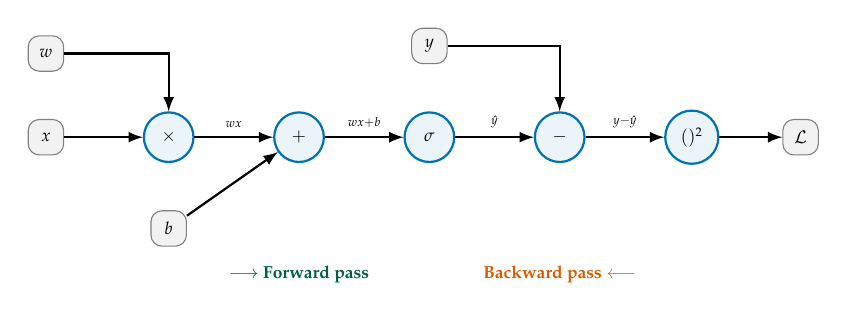
\begin{tikzpicture}[
    node distance=1.1cm,
    op/.style={circle, draw=blue, thick, minimum size=0.7cm, fill=blue!8, font=\scriptsize},
    var/.style={rectangle, draw=gray, rounded corners, minimum size=0.5cm, fill=gray!10, font=\scriptsize},
    >=latex,
    scale=0.9, every node/.style={scale=0.9}
]
    \node[var] (x) {$x$};
    \node[var, above=0.6cm of x] (w) {$w$};
    \node[op, right=1cm of x] (mul) {$\times$};
    \node[var, below=0.6cm of mul] (b) {$b$};
    \node[op, right=1cm of mul] (add) {$+$};
    \node[op, right=1cm of add] (sig) {$\sigma$};
    \node[var, above=0.6cm of sig] (y) {$y$};
    \node[op, right=1cm of sig] (sub) {$-$};
    \node[op, right=1cm of sub] (sq) {$()^2$};
    \node[var, right=0.8cm of sq] (L) {$\mathcal{L}$};

    \draw[->, thick] (x) -- (mul);
    \draw[->, thick] (w) -| (mul);
    \draw[->, thick] (mul) -- node[above, font=\tiny] {$wx$} (add);
    \draw[->, thick] (b) -- (add);
    \draw[->, thick] (add) -- node[above, font=\tiny] {$wx{+}b$} (sig);
    \draw[->, thick] (sig) -- node[above, font=\tiny] {$\hat{y}$} (sub);
    \draw[->, thick] (y) -| (sub);
    \draw[->, thick] (sub) -- node[above, font=\tiny] {$y{-}\hat{y}$} (sq);
    \draw[->, thick] (sq) -- (L);

    % Forward/backward labels below
    \node[below=1.2cm of add, font=\scriptsize, text=green!60!black] {$\longrightarrow$ \textbf{Forward pass}};
    \node[below=1.2cm of sub, font=\scriptsize, text=red] {\textbf{Backward pass} $\longleftarrow$};
\end{tikzpicture}
\end{center}

\vspace{4pt}
\begin{wideitemize}
    \item \textbf{Forward pass:} compute output left to right.
    \item \textbf{Backward pass:} compute gradients right to left using chain rule.
\end{wideitemize}
\end{frame}

% ---- Backward through the graph ----
\begin{frame}
\frametitle{Backward Pass Through the Graph}

Starting from $\mathcal{L} = (y - \hat{y})^2$, let $e = y - \hat{y}$. Work right-to-left:

\vspace{4pt}
\begin{align*}
    \pd{\mathcal{L}}{e} &= 2e = 2(y - \hat{y}) && \text{\scriptsize(derivative of square)} \\[4pt]
    \pd{\mathcal{L}}{\hat{y}} &= \pd{\mathcal{L}}{e} \cdot \pd{e}{\hat{y}} = 2(y-\hat{y}) \cdot (-1) = -2(y - \hat{y}) && \text{\scriptsize(chain rule)} \\[4pt]
    \pd{\mathcal{L}}{z} &= \pd{\mathcal{L}}{\hat{y}} \cdot \sigma'(z) = -2(y-\hat{y}) \cdot \sigma'(z) && \text{\scriptsize(through activation)} \\[4pt]
    \textcolor{red}{\pd{\mathcal{L}}{w}} &= \pd{\mathcal{L}}{z} \cdot x = \textcolor{red}{-2(y-\hat{y})\,\sigma'(z)\, x} && \text{\scriptsize(through multiplication)}
\end{align*}

\vspace{4pt}
\fbox{\textbf{Key pattern:} each node passes its gradient backward, multiplied by the local derivative.}
\end{frame}


% ============================================================
\section{Backpropagation Algorithm}
% ============================================================

\begin{transitionframe}
\begin{center}
{\Huge \textbf{Backpropagation}}\\[10pt]
{\large The engine of deep learning}
\end{center}
\end{transitionframe}

% ---- Setup ----
\begin{frame}
\frametitle{Backpropagation: Setup}

Consider a \textbf{2-layer network} (1 hidden layer):

\begin{center}
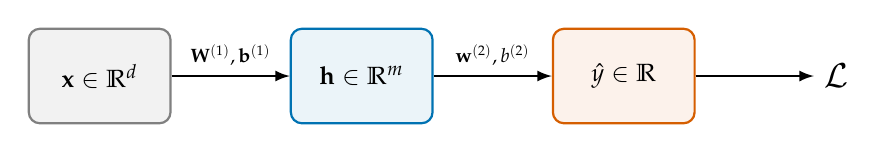
\begin{tikzpicture}[
    layer/.style={rectangle, draw=blue, thick, rounded corners, minimum height=1.2cm, minimum width=1.8cm, fill=blue!8, font=\small},
    >=latex
]
    \node[layer, fill=gray!10, draw=gray] (input) {$\vx \in \R^d$};
    \node[layer, right=1.5cm of input] (h1) {$\vh \in \R^m$};
    \node[layer, fill=red!8, draw=red, right=1.5cm of h1] (out) {$\hat{y} \in \R$};
    \node[right=1.5cm of out, font=\large] (L) {$\mathcal{L}$};

    \draw[->, thick] (input) -- node[above, font=\scriptsize] {$\vW^{(1)}, \vb^{(1)}$} (h1);
    \draw[->, thick] (h1) -- node[above, font=\scriptsize] {$\vw^{(2)}, b^{(2)}$} (out);
    \draw[->, thick] (out) -- (L);
\end{tikzpicture}
\end{center}

\textbf{Forward pass equations:}
\begin{align*}
    \vz^{(1)} &= \vW^{(1)}\vx + \vb^{(1)} && \vz^{(1)} \in \R^m \quad \text{(pre-activation)} \\
    \vh &= \sigma(\vz^{(1)}) && \vh \in \R^m \quad \text{(activation)} \\
    z^{(2)} &= (\vw^{(2)})^\top \vh + b^{(2)} && z^{(2)} \in \R \quad \text{(output logit)} \\
    \hat{y} &= z^{(2)} && \text{(for regression, no final activation)} \\
    \mathcal{L} &= (y - \hat{y})^2 && \text{(MSE loss)}
\end{align*}

\vspace{4pt}
\textbf{Goal:} Compute $\pd{\mathcal{L}}{\vW^{(1)}}$, $\pd{\mathcal{L}}{\vb^{(1)}}$, $\pd{\mathcal{L}}{\vw^{(2)}}$, $\pd{\mathcal{L}}{b^{(2)}}$.
\end{frame}

% ---- Output Layer Gradients ----
\begin{frame}
\frametitle{Backpropagation Step 1: Output Layer Gradients}

\textbf{Start from the loss} and work backward.

\vspace{6pt}
\textbf{Step 1a:} Gradient of loss w.r.t.\ output:
\[
    \pd{\mathcal{L}}{\hat{y}} = \pd{}{\hat{y}}(y - \hat{y})^2 = -2(y - \hat{y})
\]

Since $\hat{y} = z^{(2)}$: \quad $\pd{\mathcal{L}}{z^{(2)}} = -2(y - \hat{y})$. \quad Define $\textcolor{red}{\delta^{(2)} \equiv \pd{\mathcal{L}}{z^{(2)}} = -2(y - \hat{y})}$.

\vspace{8pt}
\textbf{Step 1b:} Gradient w.r.t.\ output layer parameters:
\[
    z^{(2)} = \sum_{j=1}^{m} w_j^{(2)} h_j + b^{(2)}
\]

\[
    \pd{\mathcal{L}}{w_j^{(2)}} = \delta^{(2)} \cdot \pd{z^{(2)}}{w_j^{(2)}} = \textcolor{red}{\delta^{(2)} \cdot h_j} \qquad \Rightarrow \qquad \pd{\mathcal{L}}{\vw^{(2)}} = \delta^{(2)} \cdot \vh
\]

\[
    \pd{\mathcal{L}}{b^{(2)}} = \textcolor{red}{\delta^{(2)}}
\]
\end{frame}

% ---- Hidden Layer Gradients ----
\begin{frame}
\frametitle{Backpropagation Step 2: Hidden Layer Gradients}

\textbf{Step 2a:} Propagate error back to hidden layer. Using chain rule:
\[
    \pd{\mathcal{L}}{h_j} = \delta^{(2)} \cdot \pd{z^{(2)}}{h_j} = \delta^{(2)} \cdot w_j^{(2)}
\]

\textbf{Step 2b:} Pass through the activation function:
\[
    \pd{\mathcal{L}}{z_j^{(1)}} = \pd{\mathcal{L}}{h_j} \cdot \sigma'(z_j^{(1)}) = \delta^{(2)} \cdot w_j^{(2)} \cdot \sigma'(z_j^{(1)}) \;\equiv\; \textcolor{red}{\delta_j^{(1)}}
\]

\textbf{Step 2c:} Gradients w.r.t.\ hidden layer parameters (since $z_j^{(1)} = \sum_k W_{jk}^{(1)} x_k + b_j^{(1)}$):
\[
    \pd{\mathcal{L}}{W_{jk}^{(1)}} = \delta_j^{(1)} \cdot x_k \quad \Rightarrow \quad \textcolor{red}{\pd{\mathcal{L}}{\vW^{(1)}} = \bm{\delta}^{(1)} \vx^\top}
    \qquad
    \pd{\mathcal{L}}{b_j^{(1)}} = \textcolor{red}{\delta_j^{(1)}}
\]
\end{frame}

% ---- General Backprop Formula ----
\begin{frame}
\frametitle{The General Backpropagation Formula}

Define the \textbf{error signal} at layer $l$: \quad $\bm{\delta}^{(l)} \equiv \pd{\mathcal{L}}{\vz^{(l)}}$

\vspace{6pt}
\begin{tikzpicture}
\node [mybox] (box){%
    \begin{minipage}{0.93\textwidth}
    \vspace{-4pt}
    \textbf{Output layer} ($l = L$): \quad $\bm{\delta}^{(L)} = \pd{\mathcal{L}}{\hat{\vy}} \odot \sigma'(\vz^{(L)})$

    \vspace{6pt}
    \textbf{Hidden layers} ($l = L{-}1, \ldots, 1$): \quad $\bm{\delta}^{(l)} = \left[(\vW^{(l+1)})^\top \bm{\delta}^{(l+1)}\right] \odot \sigma'(\vz^{(l)})$

    \vspace{6pt}
    \textbf{Parameter gradients:} \quad $\pd{\mathcal{L}}{\vW^{(l)}} = \bm{\delta}^{(l)} (\vh^{(l-1)})^\top$ \qquad $\pd{\mathcal{L}}{\vb^{(l)}} = \bm{\delta}^{(l)}$
    \vspace{2pt}
    \end{minipage}
};
\node[fancytitle, right=10pt] at (box.north west) {Backpropagation Equations};
\end{tikzpicture}

\vspace{8pt}
Here $\odot$ denotes element-wise (Hadamard) product and $\vh^{(0)} = \vx$.

\vspace{4pt}
\textbf{Intuition:} The error at layer $l$ is the error from layer $l{+}1$ projected back through $\vW^{(l+1)}$, scaled by how sensitive the activation was ($\sigma'$).
\end{frame}

% ---- Backprop Summary Diagram ----
\begin{frame}
\frametitle{Backpropagation: Visual Summary}

\begin{center}
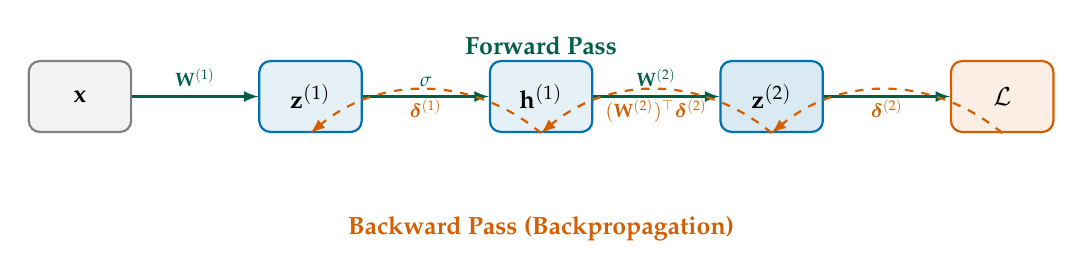
\begin{tikzpicture}[
    layer/.style={rectangle, draw, thick, rounded corners, minimum height=0.9cm, minimum width=1.3cm, font=\small},
    >=latex, node distance=1.6cm
]
    % Layers
    \node[layer, draw=gray, fill=gray!10] (x) {$\vx$};
    \node[layer, draw=blue, fill=blue!10, right=of x] (z1) {$\vz^{(1)}$};
    \node[layer, draw=blue, fill=blue!10, right=of z1] (h1) {$\vh^{(1)}$};
    \node[layer, draw=blue, fill=blue!15, right=of h1] (z2) {$\vz^{(2)}$};
    \node[layer, draw=red, fill=red!10, right=of z2] (L) {$\mathcal{L}$};

    % Forward arrows (on top)
    \draw[->, thick, green!60!black] (x) -- node[above, font=\scriptsize] {$\vW^{(1)}$} (z1);
    \draw[->, thick, green!60!black] (z1) -- node[above, font=\scriptsize] {$\sigma$} (h1);
    \draw[->, thick, green!60!black] (h1) -- node[above, font=\scriptsize] {$\vW^{(2)}$} (z2);
    \draw[->, thick, green!60!black] (z2) -- (L);

    % Backward arrows (below, well separated)
    \draw[->, thick, red, dashed] (L.south) to[bend right=40] node[below, font=\scriptsize, text=red] {$\bm{\delta}^{(2)}$} (z2.south);
    \draw[->, thick, red, dashed] (z2.south) to[bend right=40] node[below, font=\scriptsize, text=red] {$(\vW^{(2)})^\top\bm{\delta}^{(2)}$} (h1.south);
    \draw[->, thick, red, dashed] (h1.south) to[bend right=40] node[below, font=\scriptsize, text=red] {$\bm{\delta}^{(1)}$} (z1.south);

    % Labels
    \node[above=0.4cm, font=\small\bfseries, text=green!60!black] at ($(z1)!0.5!(z2)$) {Forward Pass};
    \node[below=1.4cm, font=\small\bfseries, text=red] at ($(z1)!0.5!(z2)$) {Backward Pass (Backpropagation)};
\end{tikzpicture}
\end{center}

\vspace{6pt}
\textbf{Algorithm:}
\begin{enumerate}
    \item \textcolor{green!60!black}{\textbf{Forward:}} Compute all $\vz^{(l)}$, $\vh^{(l)}$, and $\mathcal{L}$ (save intermediate values).
    \item \textcolor{red}{\textbf{Backward:}} Compute $\bm{\delta}^{(L)}, \bm{\delta}^{(L-1)}, \ldots, \bm{\delta}^{(1)}$ using the recursion.
    \item \textbf{Update:} $\vW^{(l)} \leftarrow \vW^{(l)} - \alpha \, \bm{\delta}^{(l)}(\vh^{(l-1)})^\top$ for all $l$.
\end{enumerate}
\end{frame}

% ---- Numerical Example ----
\begin{frame}
\frametitle{Backpropagation: Numerical Example (Part 1)}

\textbf{Network:} 1 input $\to$ 1 hidden (sigmoid) $\to$ 1 output (linear). MSE loss.

\vspace{4pt}
\textbf{Parameters:} $w^{(1)} = 0.5$, $b^{(1)} = 0.1$, $w^{(2)} = -0.3$, $b^{(2)} = 0.2$

\textbf{Data:} $x = 2.0$, $y = 1.0$. \qquad \textbf{Learning rate:} $\alpha = 0.1$.

\vspace{8pt}
\textbf{Forward pass:}
\begin{align*}
    z^{(1)} &= w^{(1)} x + b^{(1)} = 0.5 \cdot 2.0 + 0.1 = 1.1 \\[4pt]
    h &= \sigma(z^{(1)}) = \sigma(1.1) = \frac{1}{1 + e^{-1.1}} = 0.7503 \\[4pt]
    z^{(2)} &= w^{(2)} h + b^{(2)} = -0.3 \cdot 0.7503 + 0.2 = -0.0251 \\[4pt]
    \hat{y} &= z^{(2)} = -0.0251 \\[4pt]
    \mathcal{L} &= (y - \hat{y})^2 = (1.0 - (-0.0251))^2 = (1.0251)^2 = 1.0508
\end{align*}
\end{frame}

% ---- Numerical Example Part 2 ----
\begin{frame}
\frametitle{Backpropagation: Numerical Example (Part 2)}

\textbf{Backward pass} (work right-to-left through the network):

\vspace{2pt}
\textbf{Step 1 -- Error at output:}
\[
    \delta^{(2)} = -2(y - \hat{y}) = -2(1.0 - (-0.0251)) = \textcolor{red}{-2.0502}
\]

\textbf{Step 2 -- Output layer gradients:}
\[
    \pd{\mathcal{L}}{w^{(2)}} = \delta^{(2)} \cdot h = (-2.0502)(0.7503) = \textcolor{red}{-1.5383}
    \qquad
    \pd{\mathcal{L}}{b^{(2)}} = \delta^{(2)} = \textcolor{red}{-2.0502}
\]

\textbf{Step 3 -- Error at hidden layer:}
\[
    \delta^{(1)} = \delta^{(2)} \cdot w^{(2)} \cdot \sigma'(z^{(1)}) = (-2.0502)(-0.3)(0.7503)(1 - 0.7503) = \textcolor{red}{0.1154}
\]

\textbf{Step 4 -- Hidden layer gradients:}
\[
    \pd{\mathcal{L}}{w^{(1)}} = \delta^{(1)} \cdot x = (0.1154)(2.0) = \textcolor{red}{0.2307}
    \qquad
    \pd{\mathcal{L}}{b^{(1)}} = \delta^{(1)} = \textcolor{red}{0.1154}
\]
\end{frame}

% ---- Numerical Example Part 3 ----
\begin{frame}
\frametitle{Backpropagation: Numerical Example (Part 3)}

\textbf{Parameter update} with learning rate $\alpha = 0.1$: \quad $\theta_{\text{new}} = \theta_{\text{old}} - \alpha \cdot \text{grad}$

\vspace{4pt}
\renewcommand{\arraystretch}{1.3}
\begin{center}
{\small
\begin{tabular}{lccc}
\toprule
\textbf{Parameter} & \textbf{Old} & \textbf{Gradient} & \textbf{New} \\
\midrule
$w^{(2)}$ & $-0.3000$ & $-1.5383$ & $-0.1462$ \\
$b^{(2)}$ & $0.2000$ & $-2.0502$ & $0.4050$ \\
$w^{(1)}$ & $0.5000$ & $0.2307$ & $0.4769$ \\
$b^{(1)}$ & $0.1000$ & $0.1154$ & $0.0885$ \\
\bottomrule
\end{tabular}
}
\end{center}

\vspace{4pt}
\textbf{Verify:} Forward pass with new params $\to$ $\hat{y}_{\text{new}} = 0.2969$
\[
    \mathcal{L}_{\text{new}} = (1.0 - 0.2969)^2 = 0.4946 \quad \textcolor{green}{\text{(down from 1.0508!} \; \checkmark\text{)}}
\]

\textbf{One gradient step reduced the loss by 53\%.} Repeat this process thousands of times to train the network.
\end{frame}

% ---- Matrix Calculus ----
\begin{frame}
\frametitle{Vector and Matrix Calculus Notation}

In practice, we work with \textbf{matrices}, not individual weights.

\vspace{4pt}
\textbf{Key identities} (for layer $l$, with $\vz^{(l)} = \vW^{(l)}\vh^{(l-1)} + \vb^{(l)}$):

\begin{align*}
    \pd{\mathcal{L}}{\vW^{(l)}} &= \bm{\delta}^{(l)} (\vh^{(l-1)})^\top && \in \R^{m^{(l)} \times m^{(l-1)}} \\[2pt]
    \pd{\mathcal{L}}{\vb^{(l)}} &= \bm{\delta}^{(l)} && \in \R^{m^{(l)}} \\[2pt]
    \pd{\mathcal{L}}{\vh^{(l-1)}} &= (\vW^{(l)})^\top \bm{\delta}^{(l)} && \in \R^{m^{(l-1)}}
\end{align*}

\textbf{Why outer product?} Each $\delta_j^{(l)}$ pairs with each $h_k^{(l-1)}$: \quad $\pd{\mathcal{L}}{W_{jk}^{(l)}} = \delta_j^{(l)} \cdot h_k^{(l-1)}$.

\vspace{4pt}
\textcolor{red}{The gradient $\pd{\mathcal{L}}{\vW^{(l)}}$ has the same shape as $\vW^{(l)}$.}
\end{frame}

% ---- Backprop Complexity ----
\begin{frame}
\frametitle{Computational Cost of Backpropagation}

\begin{itemize}
    \item \textbf{Forward pass cost:} $O\!\left(\sum_{l=1}^{L} m^{(l)} m^{(l-1)}\right)$ (matrix-vector products).
    \item \textbf{Backward pass cost:} same order as forward pass.
    \item \textbf{Memory cost:} must store all $\vz^{(l)}, \vh^{(l)}$ during forward pass.
    \item \textbf{Total:} backprop is roughly \textbf{2x} the cost of the forward pass.
\end{itemize}

\vspace{4pt}
\begin{tikzpicture}
\node [mybox] (box){%
    \begin{minipage}{0.93\textwidth}
    \vspace{-4pt}
    \textbf{Before backprop} (1986): computing gradients for a network with $P$ parameters required $O(P)$ separate forward passes.

    \textbf{With backprop:} \textcolor{red}{all gradients in one backward pass}.
    \end{minipage}
};
\node[fancytitle, right=10pt] at (box.north west) {Historical Significance};
\end{tikzpicture}
\end{frame}


% ============================================================
\section{Gradient Descent Variants}
% ============================================================

\begin{transitionframe}
\begin{center}
{\Huge \textbf{Gradient Descent Variants}}
\end{center}
\end{transitionframe}

% ---- Batch GD ----
\begin{frame}
\frametitle{Batch Gradient Descent}

\textbf{Full batch gradient descent} uses \textbf{all} $N$ samples to compute the gradient:
\[
    \vw \leftarrow \vw - \alpha \cdot \frac{1}{N}\sum_{i=1}^{N} \nabla_{\vw}\ell(\vx_i, y_i; \vw)
\]

\vspace{6pt}
\textbf{Pros:}
\begin{itemize}
    \item Stable convergence, low noise.
    \item Exact gradient direction.
\end{itemize}

\vspace{4pt}
\textbf{Cons:}
\begin{itemize}
    \item Requires loading \textbf{entire dataset} into memory.
    \item Very slow for large $N$ (one update per epoch).
    \item Can get stuck in local minima (smooth trajectory).
\end{itemize}

\vspace{6pt}
\textbf{Not practical} when $N$ is large (e.g., ImageNet: $N = 1.2$ million).
\end{frame}

% ---- SGD ----
\begin{frame}
\frametitle{Stochastic Gradient Descent (SGD)}

\textbf{SGD} uses a \textbf{single random sample} per update:
\[
    \vw \leftarrow \vw - \alpha \cdot \nabla_{\vw}\ell(\vx_i, y_i; \vw) \qquad \text{where $i$ is sampled randomly}
\]

\vspace{6pt}
\begin{columns}[T]
\begin{column}{0.48\textwidth}
\textbf{Pros:}
\begin{itemize}
    \item Very fast updates.
    \item Can escape shallow local minima (noise helps!).
    \item Low memory requirement.
\end{itemize}
\end{column}

\begin{column}{0.48\textwidth}
\textbf{Cons:}
\begin{itemize}
    \item Very noisy gradient estimate.
    \item Oscillates around minimum.
    \item May never converge exactly.
\end{itemize}
\end{column}
\end{columns}

\vspace{8pt}
\textbf{Key insight:} SGD's gradient is an \textbf{unbiased estimate} of the true gradient:
\[
    \E_i\left[\nabla_{\vw}\ell(\vx_i, y_i; \vw)\right] = \frac{1}{N}\sum_{i=1}^{N}\nabla_{\vw}\ell(\vx_i, y_i; \vw) = \nabla_{\vw}\mathcal{L}(\vw)
\]
\end{frame}

% ---- Mini-Batch SGD ----
\begin{frame}
\frametitle{Mini-Batch SGD: The Best of Both Worlds}

\textbf{Mini-batch SGD} uses a random subset $\mathcal{B} \subset \{1, \ldots, N\}$ of size $B$:
\[
    \vw \leftarrow \vw - \alpha \cdot \frac{1}{B}\sum_{i \in \mathcal{B}} \nabla_{\vw}\ell(\vx_i, y_i; \vw)
\]

\vspace{6pt}
\renewcommand{\arraystretch}{1.4}
\begin{center}
\begin{tabular}{llll}
\toprule
\textbf{Method} & \textbf{Batch size} & \textbf{Noise} & \textbf{Speed} \\
\midrule
Batch GD & $B = N$ & None & Slow \\
SGD & $B = 1$ & High & Fast \\
\textcolor{red}{Mini-batch SGD} & \textcolor{red}{$B = 32, 64, 128, 256$} & \textcolor{red}{Moderate} & \textcolor{red}{Fast} \\
\bottomrule
\end{tabular}
\end{center}

\vspace{2pt}
\textbf{Why mini-batches work so well:}
\begin{itemize}
    \item GPUs handle parallel matmul --- 32 samples $\approx$ as fast as 1.
    \item Noise reduced by factor $\frac{1}{\sqrt{B}}$ vs.\ pure SGD.
    \item Typical: $B = 32, 64, 128, 256$ (powers of 2 for GPU efficiency).
\end{itemize}
\end{frame}

% ---- Epoch and Iterations ----
\begin{frame}
\frametitle{Epochs, Iterations, and Batch Size}

\begin{tikzpicture}
\node [mybox] (box){%
    \begin{minipage}{0.93\textwidth}
    \begin{itemize}
        \item \textbf{Epoch:} one complete pass through the entire dataset.
        \item \textbf{Iteration:} one parameter update (= one mini-batch).
        \item \textbf{Iterations per epoch:} $\lceil N / B \rceil$.
    \end{itemize}
    \end{minipage}
};
\node[fancytitle, right=10pt] at (box.north west) {Terminology};
\end{tikzpicture}

\vspace{8pt}
\textbf{Example:} $N = 10{,}000$ training samples, batch size $B = 100$:
\begin{itemize}
    \item Iterations per epoch: $10{,}000 / 100 = 100$.
    \item If we train for 50 epochs: $50 \times 100 = 5{,}000$ total parameter updates.
\end{itemize}

\vspace{8pt}
\textbf{Training recipe:}
\begin{enumerate}
    \item Shuffle the dataset.
    \item Split into mini-batches of size $B$.
    \item For each mini-batch: forward $\to$ loss $\to$ backward $\to$ update.
    \item Repeat for multiple epochs.
\end{enumerate}
\end{frame}

% ---- Momentum ----
\begin{frame}
\frametitle{SGD with Momentum}

Pure SGD oscillates due to noisy gradients. \textbf{Momentum} smooths the trajectory:

\begin{tikzpicture}
\node [mybox] (box){%
    \begin{minipage}{0.93\textwidth}
    \vspace{-6pt}
    \[
        \mathbf{v}_t = \beta \mathbf{v}_{t-1} + \nabla_{\vw}\mathcal{L}(\vw_t) \qquad \vw_{t+1} = \vw_t - \alpha \mathbf{v}_t
    \]
    \vspace{-8pt}
    where $\beta \in [0, 1)$ is the momentum coefficient (typically $\beta = 0.9$).
    \end{minipage}
};
\node[fancytitle, right=10pt] at (box.north west) {Momentum Update};
\end{tikzpicture}

\vspace{4pt}
\textbf{Intuition:} a ball rolling down a hill. Momentum accumulates past gradients, so it ``rolls through'' small bumps.

\vspace{2pt}
\begin{columns}[T]
\begin{column}{0.48\textwidth}
\centering
\textcolor{blue}{\textbf{Without momentum}}

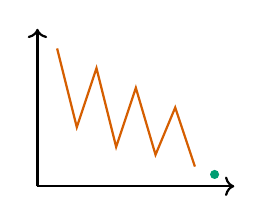
\begin{tikzpicture}[scale=0.5]
    \draw[thick, ->] (0,0) -- (5,0);
    \draw[thick, ->] (0,0) -- (0,4);
    \draw[thick, red] (0.5, 3.5) -- (1, 1.5) -- (1.5, 3) -- (2, 1) -- (2.5, 2.5) -- (3, 0.8) -- (3.5, 2) -- (4, 0.5);
    \draw[fill=green, green] (4.5, 0.3) circle (0.1);
\end{tikzpicture}

{\small Oscillates, slow convergence.}
\end{column}

\begin{column}{0.48\textwidth}
\centering
\textcolor{blue}{\textbf{With momentum}}

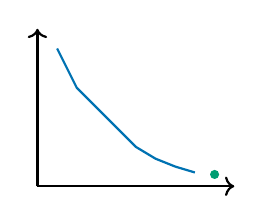
\begin{tikzpicture}[scale=0.5]
    \draw[thick, ->] (0,0) -- (5,0);
    \draw[thick, ->] (0,0) -- (0,4);
    \draw[thick, blue] (0.5, 3.5) -- (1, 2.5) -- (1.5, 2) -- (2, 1.5) -- (2.5, 1) -- (3, 0.7) -- (3.5, 0.5) -- (4, 0.35);
    \draw[fill=green, green] (4.5, 0.3) circle (0.1);
\end{tikzpicture}

{\small Smoother, faster convergence.}
\end{column}
\end{columns}
\end{frame}


% ============================================================
\section{PyTorch Implementation}
% ============================================================

\begin{transitionframe}
\begin{center}
{\Huge \textbf{PyTorch Implementation}}
\end{center}
\end{transitionframe}

% ---- PyTorch Backprop ----
\begin{frame}[fragile]
\frametitle{Backpropagation in PyTorch: Under the Hood}

\textbf{PyTorch does backpropagation automatically} via \texttt{autograd}.

\begin{lstlisting}
import torch
import torch.nn as nn

# 2-layer network: 3 inputs -> 4 hidden (ReLU) -> 1 output
model = nn.Sequential(
    nn.Linear(3, 4),     # W1: 4x3, b1: 4 -> 16 params
    nn.ReLU(),
    nn.Linear(4, 1))     # W2: 1x4, b2: 1 -> 5 params (Total: 21)

# Forward pass + loss
x = torch.randn(1, 3); y_true = torch.tensor([[1.0]])
loss = nn.MSELoss()(model(x), y_true)

# Backward pass -- ALL gradients computed automatically!
loss.backward()

for name, param in model.named_parameters():
    print(f"{name}: grad shape = {param.grad.shape}")
\end{lstlisting}
\end{frame}

% ---- Full Training ----
\begin{frame}[fragile]
\frametitle{Full Training Example: Economic Data}

\begin{lstlisting}
import torch
import torch.nn as nn
from torch.utils.data import DataLoader, TensorDataset

# Simulated economic data: 3 features -> outcome
X = torch.randn(1000, 3)
y = (2*X[:,0] - X[:,1] + 0.5*X[:,2] + torch.randn(1000)*0.1).unsqueeze(1)

# Mini-batch DataLoader
loader = DataLoader(TensorDataset(X, y), batch_size=32, shuffle=True)

# Model, loss, optimizer
model = nn.Sequential(nn.Linear(3, 16), nn.ReLU(),
                      nn.Linear(16, 8), nn.ReLU(), nn.Linear(8, 1))
criterion = nn.MSELoss()
optimizer = torch.optim.SGD(model.parameters(), lr=0.01, momentum=0.9)

# Training loop
for epoch in range(50):
    for X_batch, y_batch in loader:
        loss = criterion(model(X_batch), y_batch)
        optimizer.zero_grad(); loss.backward(); optimizer.step()
\end{lstlisting}
\end{frame}

% ---- Visualizing Loss ----
\begin{frame}[fragile]
\frametitle{Visualizing the Training Loss}

\begin{lstlisting}
import matplotlib.pyplot as plt

losses = []
for epoch in range(100):
    epoch_loss = 0
    for X_batch, y_batch in loader:
        loss = criterion(model(X_batch), y_batch)
        optimizer.zero_grad(); loss.backward(); optimizer.step()
        epoch_loss += loss.item()
    losses.append(epoch_loss / len(loader))

plt.plot(losses); plt.xlabel('Epoch'); plt.ylabel('MSE Loss')
plt.title('Training Loss Curve'); plt.grid(True); plt.show()
\end{lstlisting}

\textbf{What to look for:} loss should decrease; oscillations $\Rightarrow$ LR too large; slow decrease $\Rightarrow$ LR too small.
\end{frame}


% ============================================================
\section{Summary and Next Steps}
% ============================================================

\begin{transitionframe}
\begin{center}
{\Huge \textbf{Summary \& Next Steps}}
\end{center}
\end{transitionframe}

% ---- Summary ----
\begin{frame}
\frametitle{Summary}

\begin{enumerate}
    \item \textbf{Activation function derivatives} are critical for backprop. Sigmoid: $\sigma' = \sigma(1-\sigma)$. ReLU: $\sigma' = \mathbf{1}[z > 0]$.

    \item \textbf{Vanishing gradients:} sigmoid derivative $\leq 0.25$ causes exponential decay in deep nets. ReLU solves this.

    \item \textbf{Softmax} extends binary classification to $K$ classes: $\hat{y}_k = \frac{e^{z_k}}{\sum_j e^{z_j}}$.

    \item \textbf{Cross-entropy + softmax/sigmoid} gives gradient $\pd{\mathcal{L}}{z_i} = \hat{y}_i - y_i$.

    \item \textbf{Backpropagation} = chain rule applied layer by layer:
    \[
        \bm{\delta}^{(l)} = [(\vW^{(l+1)})^\top \bm{\delta}^{(l+1)}] \odot \sigma'(\vz^{(l)}) \qquad \pd{\mathcal{L}}{\vW^{(l)}} = \bm{\delta}^{(l)}(\vh^{(l-1)})^\top
    \]

    \item \textbf{Mini-batch SGD} with momentum is the standard optimizer. Typical $B = 32$--$256$.
\end{enumerate}
\end{frame}

% ---- Next Lecture ----
\begin{frame}
\frametitle{Next Lecture: SGD, Regularization \& Generalization}

\textbf{Lecture 3} (Monday, April 20):
\begin{itemize}
    \item Advanced optimizers: Adam, AdaGrad, RMSProp.
    \item Regularization: L1, L2 (weight decay), dropout.
    \item Batch normalization.
    \item Universal Approximation Theorem; why depth matters.
    \item Practical tips: LR schedules, early stopping.
\end{itemize}

\vspace{6pt}
\textbf{Recommended reading:} Goodfellow et al., \textit{Deep Learning}, Ch.\ 6.5 + Ch.\ 8. Zhang et al., \textit{D2L}, Ch.\ 5 (\url{https://d2l.ai}).

\vspace{6pt}
\textbf{Homework 1} will be released after Lecture 3 (due Sunday, April 27).

\vspace{4pt}
\begin{center}
\Large \textcolor{blue}{\textbf{Questions?}}
\end{center}
\end{frame}

% ---- References ----
\begin{frame}
\frametitle{References}

\small
\begin{wideitemize}
    \item Goodfellow, I., Bengio, Y., \& Courville, A. (2016). \textit{Deep Learning}. MIT Press. Chapters 6, 8.
    \item Zhang, A., Lipton, Z. C., Li, M., \& Smola, A. J. (2023). \textit{Dive into Deep Learning}. Cambridge University Press.
    \item Rumelhart, D. E., Hinton, G. E., \& Williams, R. J. (1986). Learning representations by back-propagating errors. \textit{Nature}, 323(6088), 533--536.
    \item Glorot, X., \& Bengio, Y. (2010). Understanding the difficulty of training deep feedforward neural networks. \textit{AISTATS}.
    \item Nair, V., \& Hinton, G. E. (2010). Rectified linear units improve restricted Boltzmann machines. \textit{ICML}.
    \item Kingma, D. P., \& Ba, J. (2015). Adam: A method for stochastic optimization. \textit{ICLR}.
\end{wideitemize}
\end{frame}


\end{document}
